\documentclass[11pt,dvipdfm]{article}
%\documentclass[11pt]{article}
%\usepackage[utf8]{inputenc}

\usepackage{deauthor,times,graphicx,subfig,tablefootnote,multirow,amsmath}

\graphicspath{{submissions/rep-nli-shao/}}


\begin{document}
\title{Structured Data Representation in Natural Language Interfaces}
\author{Yutong Shao,~~Arun Kumar,~~and~~Ndapa Nakashole\\
University of California, San Diego, USA\\
\texttt{\{yshao,arunkk,nnakashole\}@eng.ucsd.edu}}
\maketitle

\begin{abstract}
A Natural Language Interface (NLI)  enables the  use of human languages to interact with computer systems,  including smart phones and robots. Compared to other types of interfaces, such as  command line interfaces (CLIs) or graphical user interfaces (GUIs), NLIs stand to enable more people to have access to functionality behind databases or APIs as they only require knowledge of natural languages. Many NLI applications involve structured data for the domain (e.g., applications such as hotel booking, product search, and factual question answering.) Thus, to fully process user questions, in addition to natural language comprehension, understanding of structured data is also crucial for the model.
In this paper, we study neural network methods for building Natural Language Interfaces (NLIs) with a  focus on learning structure data representations that can generalize to novel  data sources and schemata not seen at training time. Specifically, we review two  tasks related to natural language interfaces: i) semantic parsing where we  focus on text-to-SQL  for database access,  and ii) task-oriented dialog  systems for API access. We survey representative methods for   text-to-SQL and  task-oriented dialog tasks,  focusing  on representing and incorporating structured data. Lastly, we  present two of our original studies on structured data representation methods for NLIs  to enable access to i)  databases, and ii) visualization APIs.
\end{abstract}

\section{Introduction}

Natural Language Interfaces (NLIs) seek to enable user-system interactions using natural language. Compared to other types of interfaces, such as command-line or graphic interfaces, NLIs have a much lower learning curve. They can be used by lay users with little to no extra training, thus attractive in practice.

NLIs have been an active research for decades~\cite{winograd1971procedures,karamcheti-etal-2020-learning}.
Early methods had limited success, possibly due to the absence of powerful and effective models for language understanding. Recently, with the rise of deep learning models, especially Transformer-based models in NLP~\cite{vaswaniTransformer}, the overall performance on a variety of language understanding tasks, including NLI-related tasks, has seen a significant boost. Nonetheless, the state-of-the-art (SOTA) NLI models are still far from perfect, and are do not yet reach the level of being fully deployable in real products. 
In this work, we investigate the progress and challenges of NLI-related tasks. Specifically,
we focus on two types of tasks: \textit{semantic parsing} and \textit{task-oriented dialogs (TOD)}. 
In addition, we focus on the understanding and representation of \textit{structured data}, such as knowledge bases (KBs), databases (DBs) or tables, in NLI-related tasks. In practice, NLI applications inevitably need to incorporate and understand the relevant ``backend'' structured data for the domain (hotel booking, product searching, factual question answering, etc.)
Thus, besides language comprehension, a correct understanding of structured data is also crucial for the model to make the correction decisions.

In following sections, we first provide a more detailed descriptions of the NLI-related tasks we study. For each task, we survey representative methods for the tasks, especially regarding structured data representation; then we introduce our own work related to the task. A road map of this paper is illustrated in Figure~\ref{fig:roadmap}.

\begin{figure}[h]
\centering
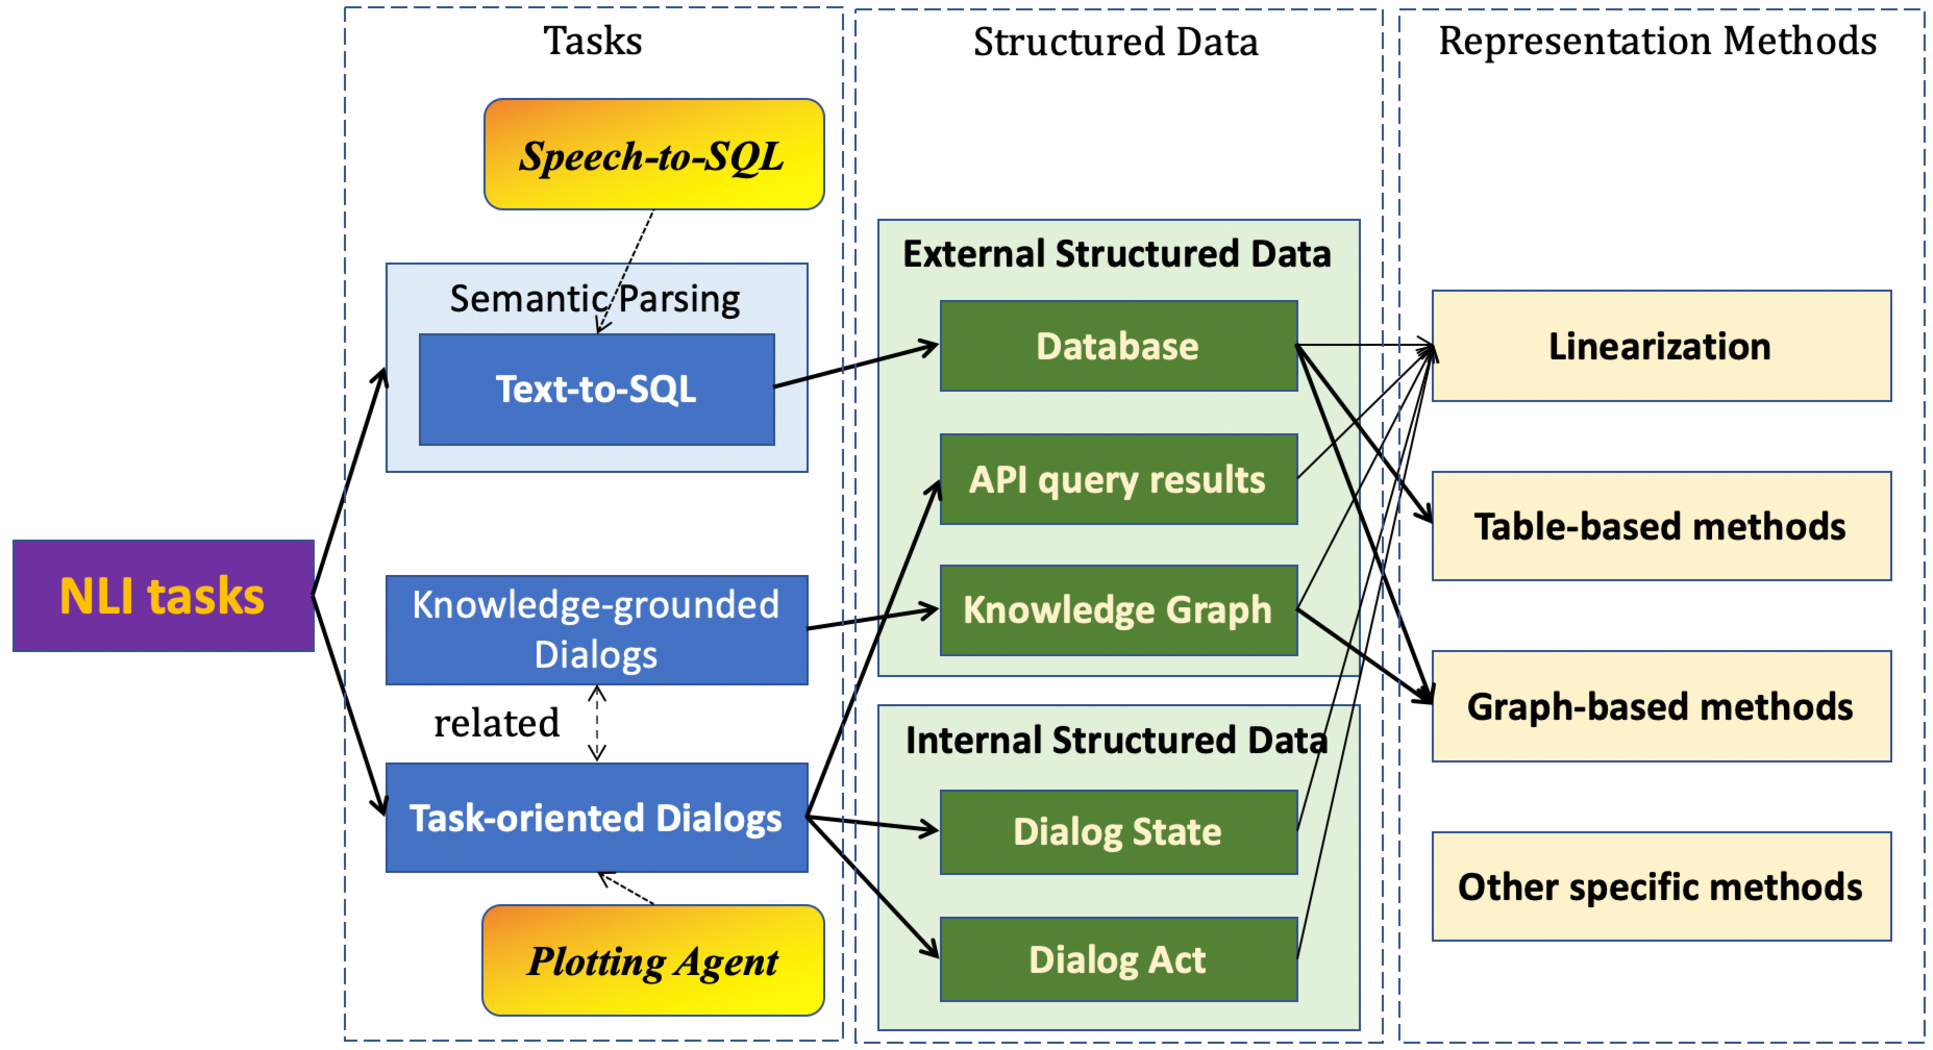
\includegraphics[width=0.6\textwidth]{figs/roadmap-v1.1.pdf}
% 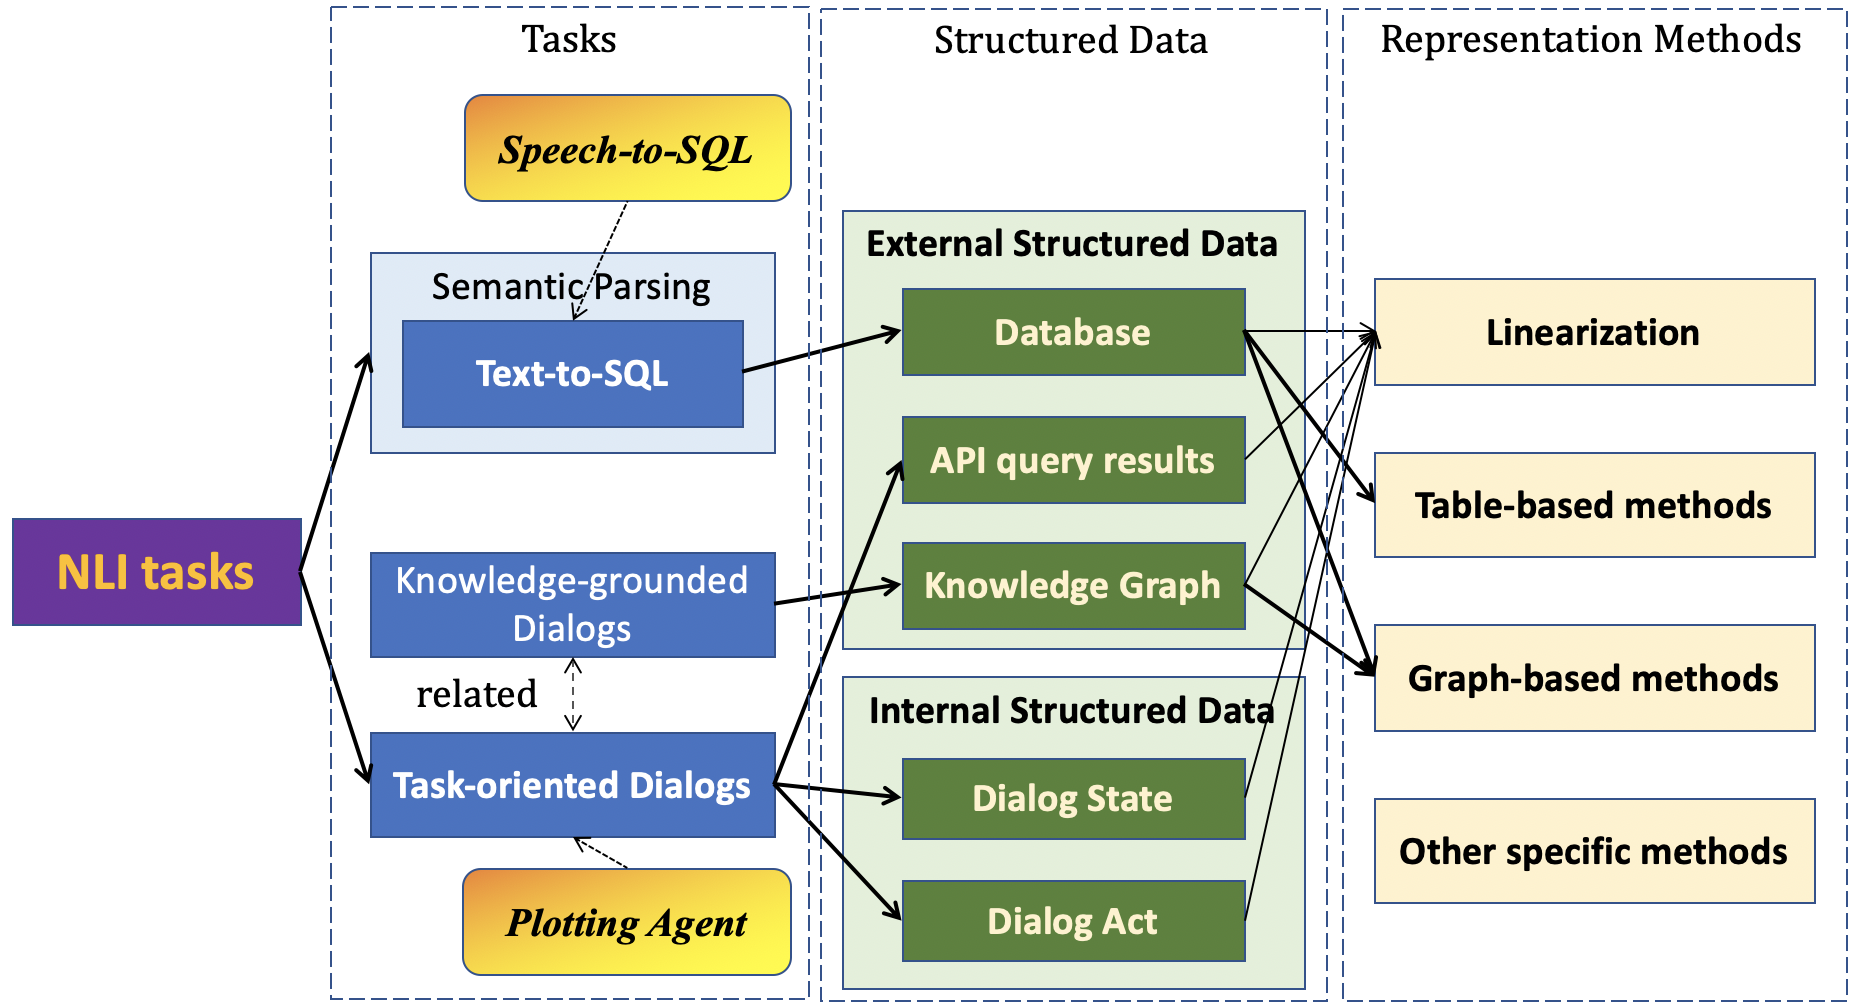
\includegraphics[bb= 0 0 1392 756, width=0.6\textwidth]{figs/roadmap-v1.1.png}
% 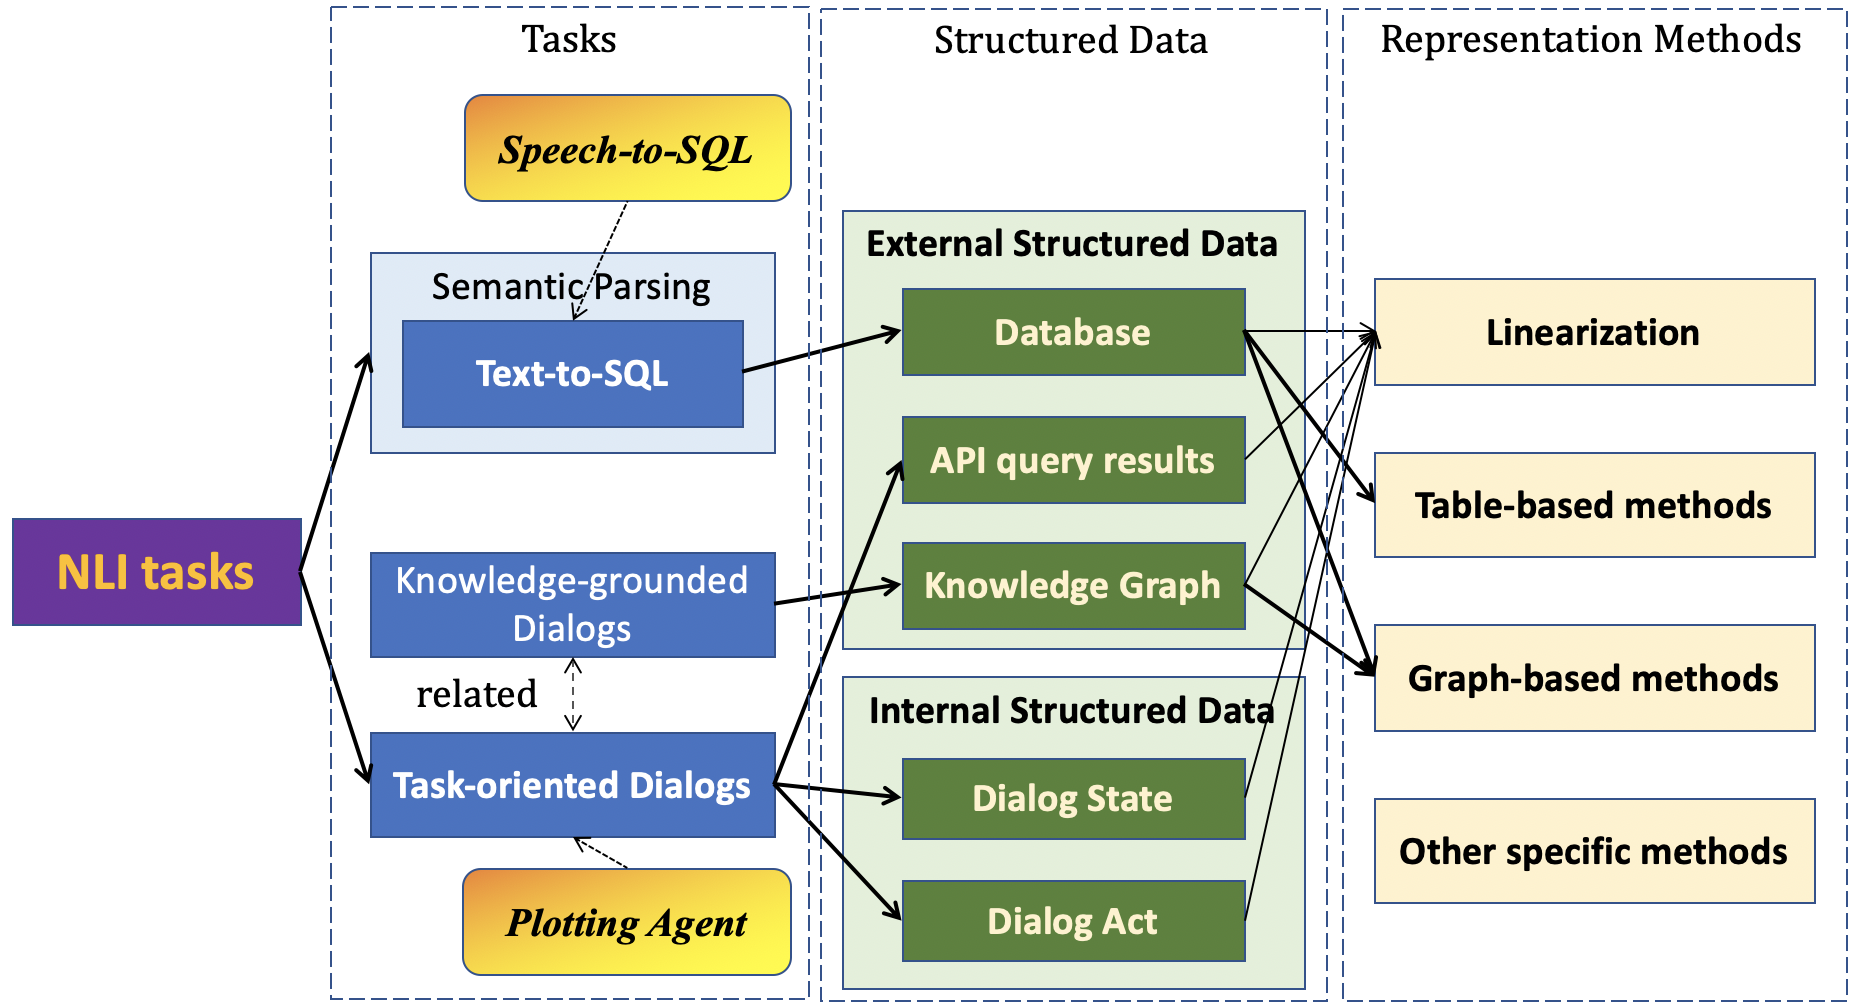
\includegraphics[bb= 0 0 928 504, width=0.6\textwidth]{figs/roadmap-v1.1.png}
\caption{The road map of the paper. We discuss several NLI-related tasks, relevant structured data and corresponding representation methods. We introduce two of our own related work, Speech-to-SQL and Plotting Agent, under the topic.}
\label{fig:roadmap}
\end{figure}


\section{Preliminaries}
\subsection{Popular NLP models}
We briefly introduce several model architectures that are widely used today in the NLP community and will be frequently mentioned in this paper.

\paragraph{Sequence-to-sequence (S2S)} A sequence-to-sequence (S2S) model aims to map an input sequence to an output sequence~\cite{seq2seq}. In NLP, the input and output sequences are usually natural language sentences. Many NLP tasks can be modeled by S2S models, such as machine translation, summarization,  and dialog.
%etc.

S2S models are mostly based on an \textit{encoder-decoder} model architecture, in which the \textit{encoder} aims to obtain an intermediate vector or tensor representation that includes necessary information from the input sequence (named the \textit{encoding} of input), and the \textit{decoder} generates the output sentence based on the input encoding. Both encoder and decoder can be modeled by recurrent neural networks (RNNs), such as LSTM or GRU~\cite{lstm,gru}; or by transformer models, which we briefly introduce below.

% Figure~\ref{fig:prelim-encdec-base} illustrates the basic version of RNN-based S2S model architecture.
%%Ndapa: we should skip these figures and refer the reader to the original papers for further details on the preliminaries.
%% Figures "define" and give an identity to a paper, and we don't want these figures to define our work since people have seen them too many times.

In the  basic version of RNN-based S2S model architecture,the encoder absorbs an input sentence and encodes it into a single \textit{encoding vector}; the decoder takes the encoding vector to generate an output sentence as a conditioned language model (i.e. generate tokens in auto-regressive manner, based on previous tokens). Intuitively, the encoding vector is an information bottleneck in the architecture because all information from the input has to be incorporated into a single vector.

\paragraph{Attention} The attention mechanism~\cite{bahdanauAttention,luongAttention} was proposed to overcome the above-mentioned bottleneck. It allows the decoder states to ``look through'' the encoding vector and directly interact with encoder states. In detail, given a decoder state vector $d$ and encoder state vectors $e_{1:N}$, we compute an \textit{attention context vector} $c$ as follow:
% \begin{gather*}
$$
    \alpha_k = \frac{\texttt{sim}(d,e_k)}{\sum_{i=1}^{N}\texttt{sim}(d,e_i)} \\
    ;
    c = \sum_{k=1}^{N}\alpha_k e_k
$$
% \end{gather*}
where $\alpha_k$ are called \textit{attention weights}, and \texttt{sim} is a function measuring vector similarities, such as dot product ($a^Tb$), bilinear product ($a^TWb$), linear combination ($w_1^Ta+w_2^Tb$), etc. The attention context vector is then added or concatenated with the decoder state vector before predicting the output token.


% \begin{figure}[h]
% \centering
% \subfloat[Basic S2S model.]{\label{fig:prelim-encdec-base}{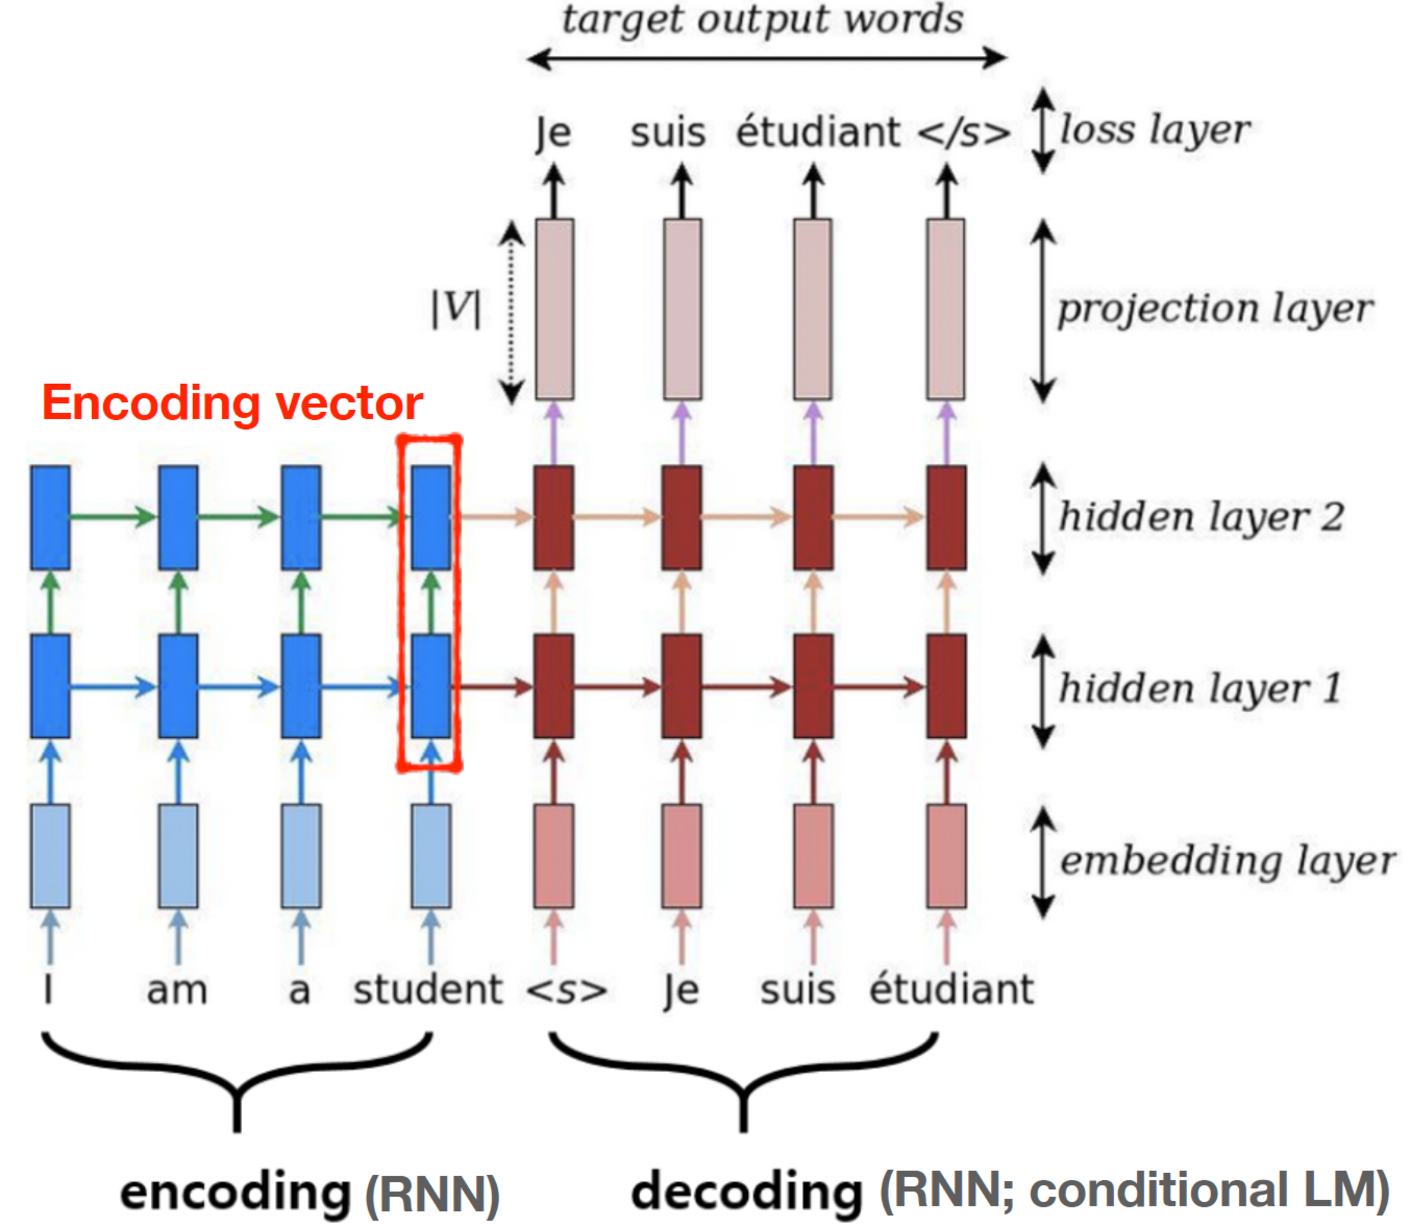
\includegraphics[width=0.45\linewidth]{figs/EncDec.pdf}}}~
% \subfloat[S2S model with attention mechanism.]{\label{fig:prelim-encdec-att}{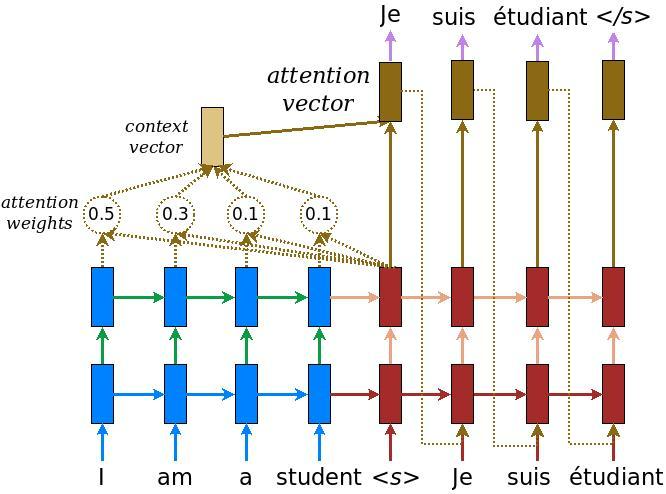
\includegraphics[width=0.45\linewidth]{figs/EncDec-att.png}}}
% % \vspace{0.2cm}
% \caption{Sequence-to-sequence (S2S) model with encoder-decoder architecture (figures from~\cite{tensorflowNMT}).}
% \label{fig:prelim-encdec}
% \end{figure}

\paragraph{Self-attention and Transformers} The Transformer architecture, proposed in \cite{vaswaniTransformer}, fully replaces RNNs with \textit{self-attention} layers. Self-attention layers encode a sequence by applying attention from the representation of each token to all other tokens in the sequence, and use the attention context vector (with residual connection, i.e. summed with the pre-attention representation vector) as the output token representation. 
% An illustration of transformer architecture is shown in Figure~\ref{fig:transformer}. 
Transformers are shown to be particularly useful for pretrained language models (PLMs), i.e. first \textit{pretrain} the model on an extremely large corpus with self-supervision, and then \textit{fine-tune} the pretrained parameters on a downstream task~\cite{bert,gpt2}.

% \begin{figure}[h]
% \centering
% 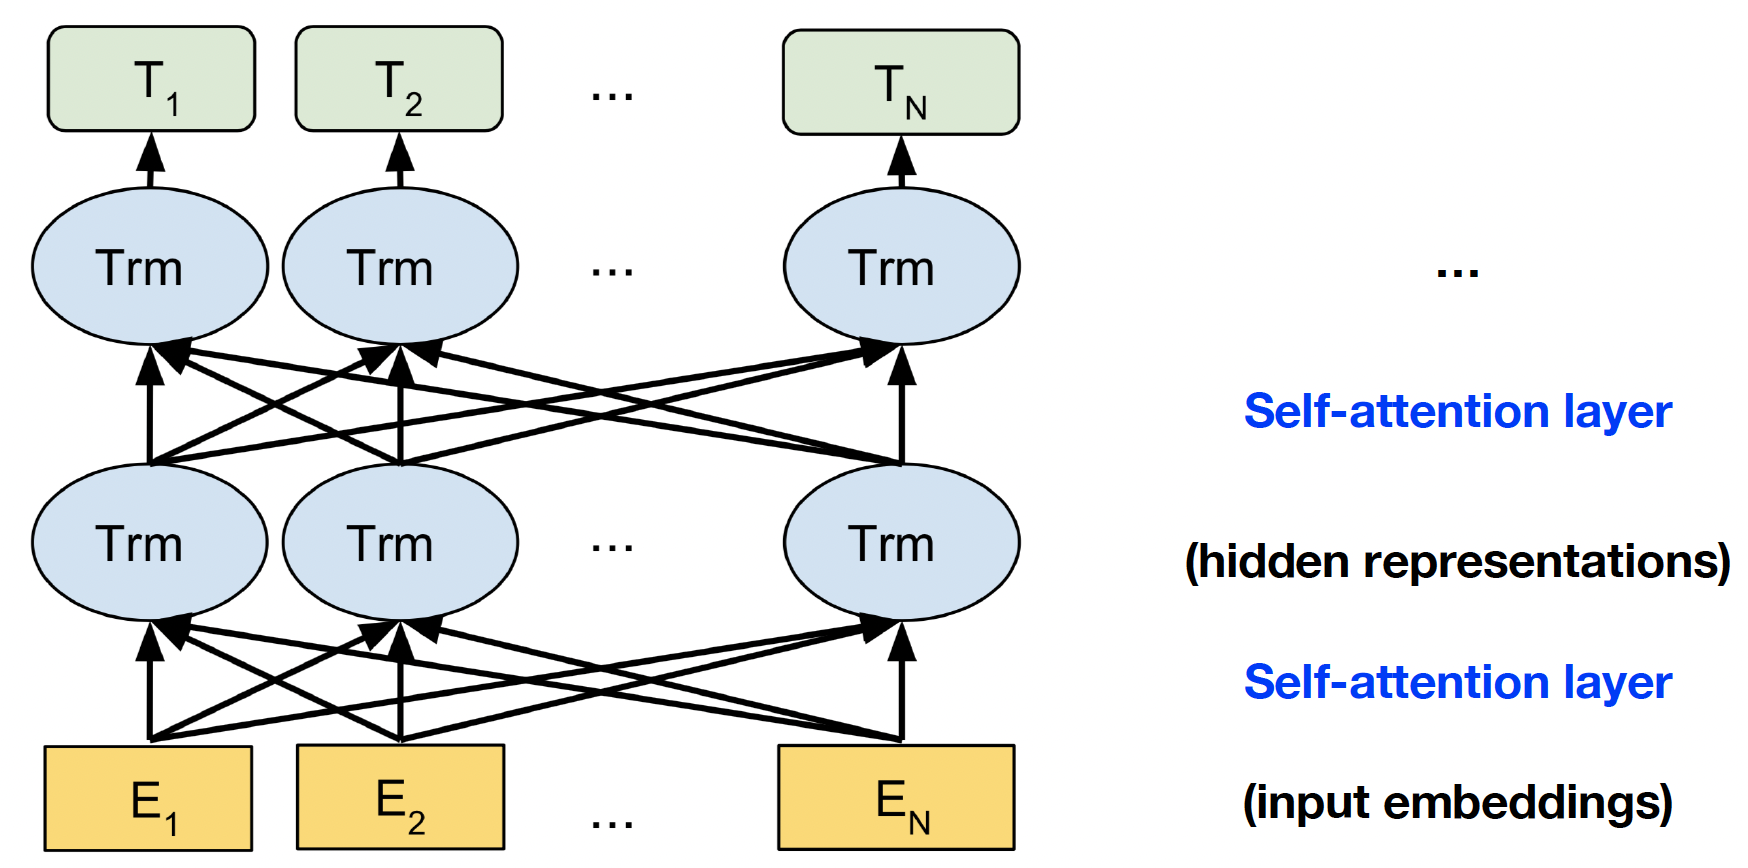
\includegraphics[width=0.45\linewidth]{figs/transformer.png}
% \caption{The Transformer architecture (imported from~\cite{bert}).}
% \label{fig:transformer}
% \end{figure}

% \section{Related Tasks}
\subsection{NLI-related Tasks}
The topic of NLIs is broad.
%highly inclusive. 
In this work, we 
focus on two representative tasks: semantic parsing and task-oriented dialogs (TOD). These tasks are useful in practice and widely studied, especially in the current era of deep learning. We briefly introduce the tasks in this section and take in-depth investigations in the following sections.

% \yutongtodo{A roadmap figure} %% I think we should put the roadmap figure at the end of the intro??

\paragraph{Semantic Parsing}
Semantic parsing aims to map a natural language sentence into a structured, executable logical form to represent the semantics of the sentence. It can be seen as a straightforward formulation of an NLI: parsing the natural language query into system-understandable form.
% The backend system provides a set of executable functions, which can be used in the logical forms. Figure \ref{fig:geo-logical-form} shows several sample pairs of sentence and logical form.
% The study of semantic parsing can date back to very early work such as the GeoQuery dataset with the CHILL system \cite{GeoQuery:Zelle1996LearningTP}, which is a grammar-based shift-reduce parser.
There are different formats of such executable logical forms, such as GeoQuery~\cite{GeoQuery:Zelle1996LearningTP},
%% \yutong{any name for GeoQuery logical form?}
lambda-DCS~\cite{WTQ}, SparQL (for knowledge graphs (KG)) and SQL (for relational databases (DB)).
% We show examples of semantic parsing in Figure~\ref{fig:geoquery-samples}.


% \begin{figure}[h]
% \centering
% 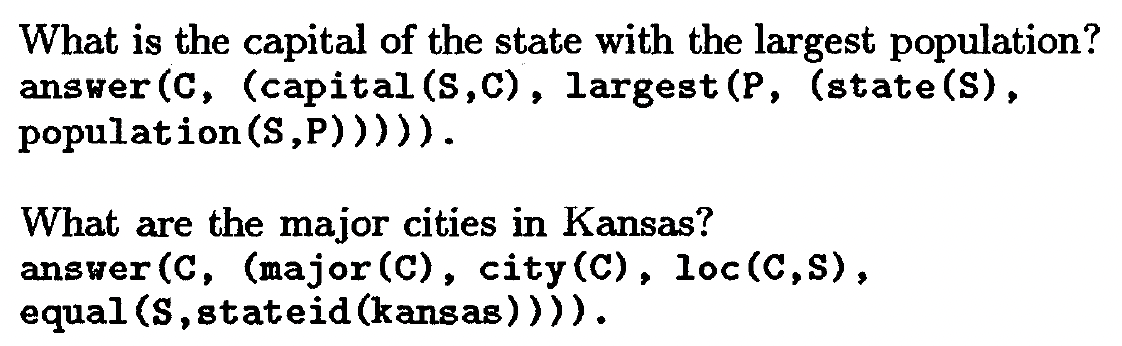
\includegraphics[width=0.45\linewidth]{figs/geoquery-samples.png}
% \caption{Samples of semantic parsing (imported from~\cite{GeoQuery:Zelle1996LearningTP}).}
% \label{fig:geoquery-samples}
% \end{figure}


% \begin{figure}[ht]
% \centering
% \subfloat[A]{\label{fig:overall-ugt}{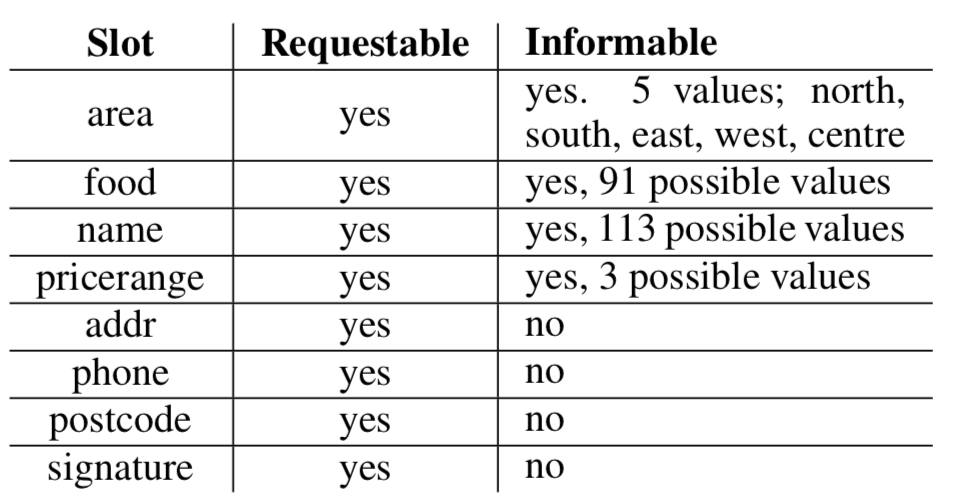
\includegraphics[width=0.24\textwidth]{figs/DSTC2-onto.png}}}
% \subfloat[B]{\label{fig:overall-wct}{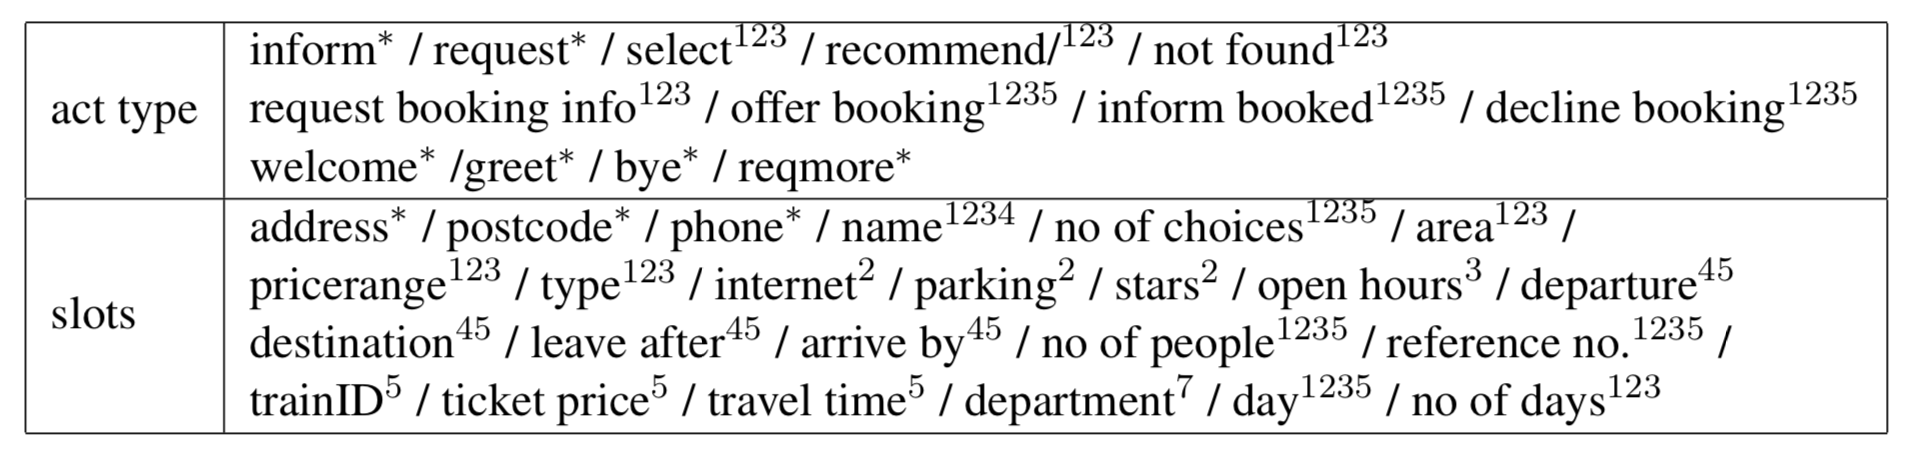
\includegraphics[width=0.24\textwidth]{figs/MultiWOZ-onto.png}}}
% \vspace{0.2cm}
% \caption{{Overall MAP@$k_g$ performance of each method on (a) user-generated text and (b) well-curated benchmarks. SOTA methods (CGExpan, SetExpan) are outperformed by simple baselines and ensemble methods on X.
% }}
% \label{fig:overall-results}
% %\vspace{-10pt}
% \end{figure}


\paragraph{Task-oriented Dialog (TOD)}
Task-oriented dialog (TOD) systems interact with users to complete certain tasks. The task objectives are usually in the form of making API calls to obtain information (e.g. look for restaurants) or take actions (e.g. make a restaurant reservation)~\cite{bAbIDialog,airdialogue,DSTC2,multiwoz}. From a practical perspective, for complex tasks, it is hard for user requests to be described and completed in a single utterance. Therefore, interactions are necessary between the user and system to complete the task, which makes a task-oriented dialog. 
% Several sample dialogs are shown in Figure~\ref{fig:babi-sample}.

% \begin{figure}[h]
% \centering
% 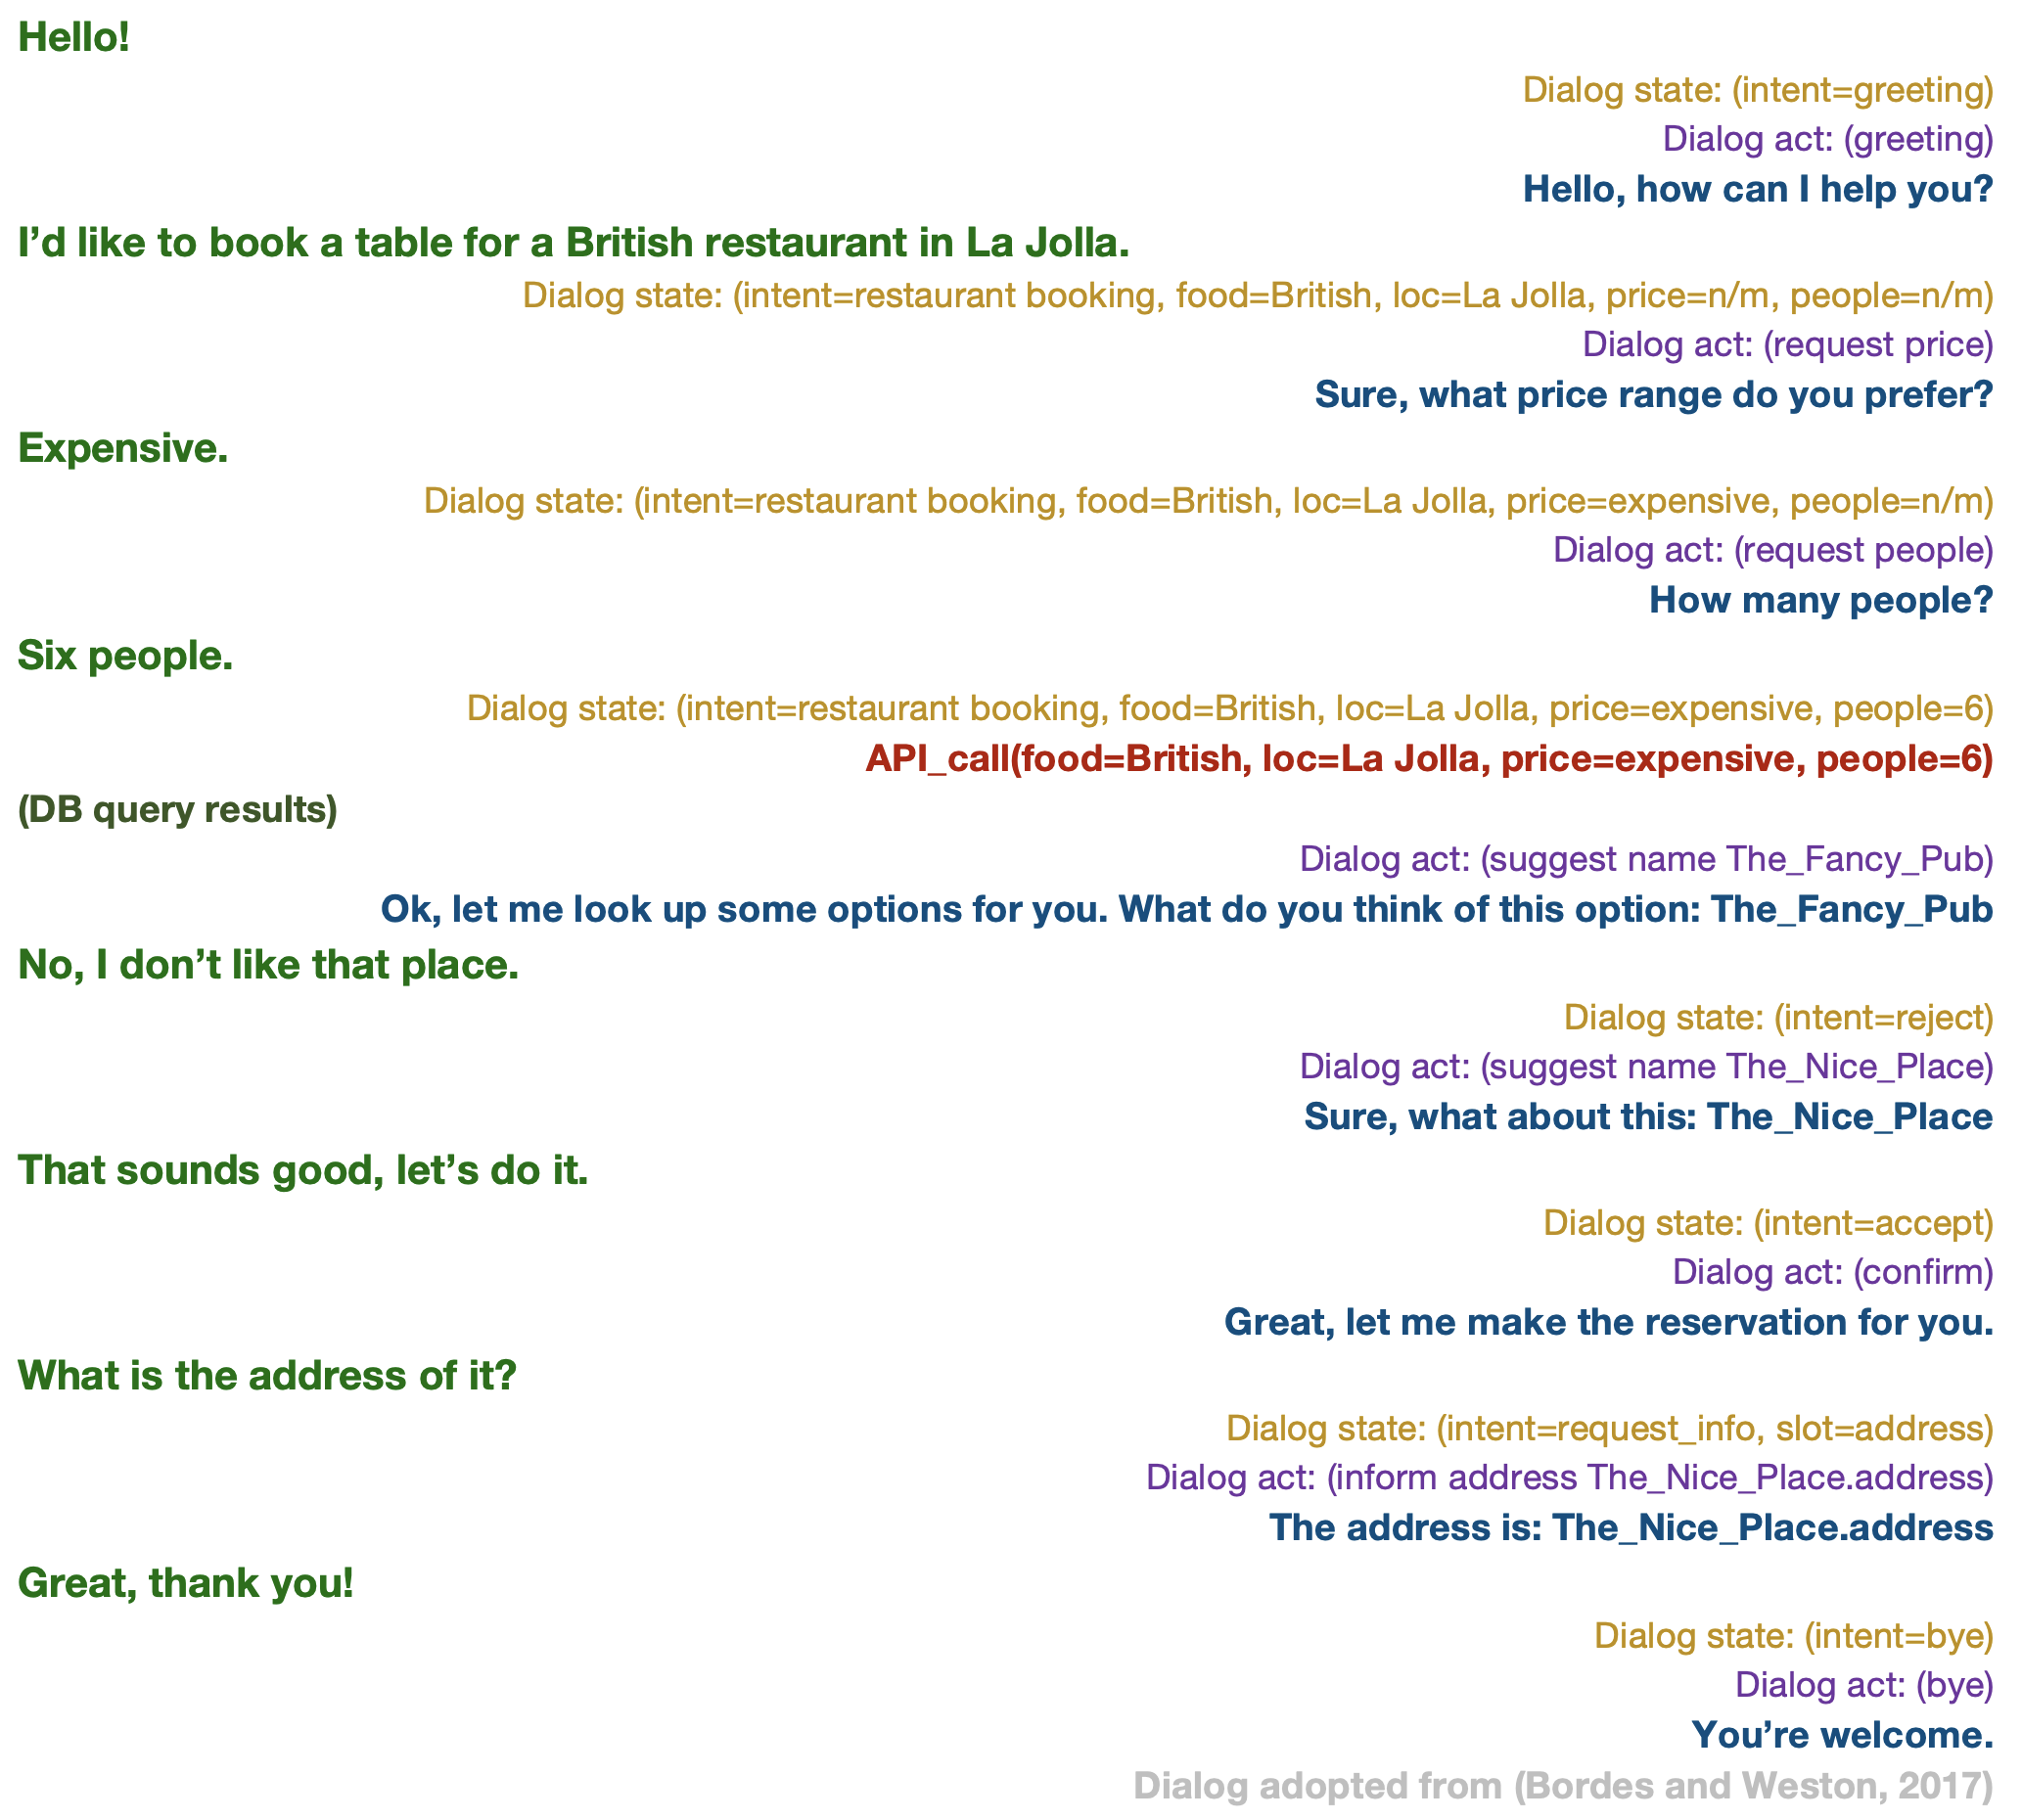
\includegraphics[width=0.55\linewidth]{figs/babi-tod.png}
% \caption{An example task-oriented dialog (TOD). On the left are input (user utterances or DB query results); on the right are system predictions, including dialog state, dialog act and response. (adopted from~\cite{bAbIDialog}).}
% \label{fig:babi-sample}
% \end{figure}


\section{Semantic Parsing}

\subsection{Introduction}
Early work in semantic parsing are based on grammar rules induction and feature-based rule selection~\cite{GeoQuery:Zelle1996LearningTP,Artzi2013UWSPF}.
Since the rise of deep learning, parsers are mostly based on neural models with encoder-decoder architectures that generate the output logical form directly from input text \cite{Dong2016LanguageTL,Dong2018CoarsetoFineDF,Cheng2019LearningAE}.
Moreover, recent work pay increasingly more attention on the \textit{generalization ability} of trained models, especially on generalizing over changes in the backend structured data. The advantages of such generalization is to alleviate the burden of re-collecting in-domain data and re-training the model whenever we update our DB or KG. In order to generalize to unseen structured data, we have to incorporate the structured data as part of the input to the model, instead of fully include them into the model weights. It thus raises the problem of \textit{structured data representation}, which is basically on how to effectively incorporate and leverage the structured data for a better model performance.

In what follows, we focus on structured data representation on semantic parsing with SQL as the logical form, which is also called text-to-SQL. As mentioned, the task of text-to-SQL takes as input the user utterance in natural language and the backend DB. A recent benchmark on text-to-SQL, Spider~\cite{yu2018spider}, explicitly tests the generalization ability to unseen DBs by separating the set of DBs used in train/dev/test splits of the benchmark. It provides a good testbed for modern text-to-SQL methods and has been widely used by previous work in this direction. 

\subsection{Structured Data Representation in Text-to-SQL}
\subsubsection{Basic Method: Linearization}
In the task of text-to-SQL, the structured data to be incorporated are the DBs.
% There are three types of method to represent DBs: table-based, graph-based and linearization.
The most straightforward idea is to \textit{linearize} the DB, i.e. transform it into a token sequence, and concatenate it with the user question to form the input text. A simple example is shown in Figure~\ref{fig:db-linearize}. By linearizing, the structured data is mapped into unstructured text modality, thus can fit into regular text-processing models.

Despite of its simplicity, linearization has shown to be a very useful way to represent DBs~\cite{picard,uskg}. There are also work focusing on injecting more useful information into such linear representations. For example, in~\cite{bridge} the authors propose to find \textit{anchor text} which are input text tokens matching DB cell values, and add them to the linearized DB, next to the column of the cell (similar to the format of cell inclusion shown in Figure~\ref{fig:db-linearize}). Also, DB linearization works well with large-scale pretraining~\cite{grappa,tabert}. This is possibly due to the compatibility of linearized DB and unstructured text, thus effective pretraining objectives (such as masked language-modeling (MLM)) can be adopted.

% \begin{figure}[h]
% \centering
% 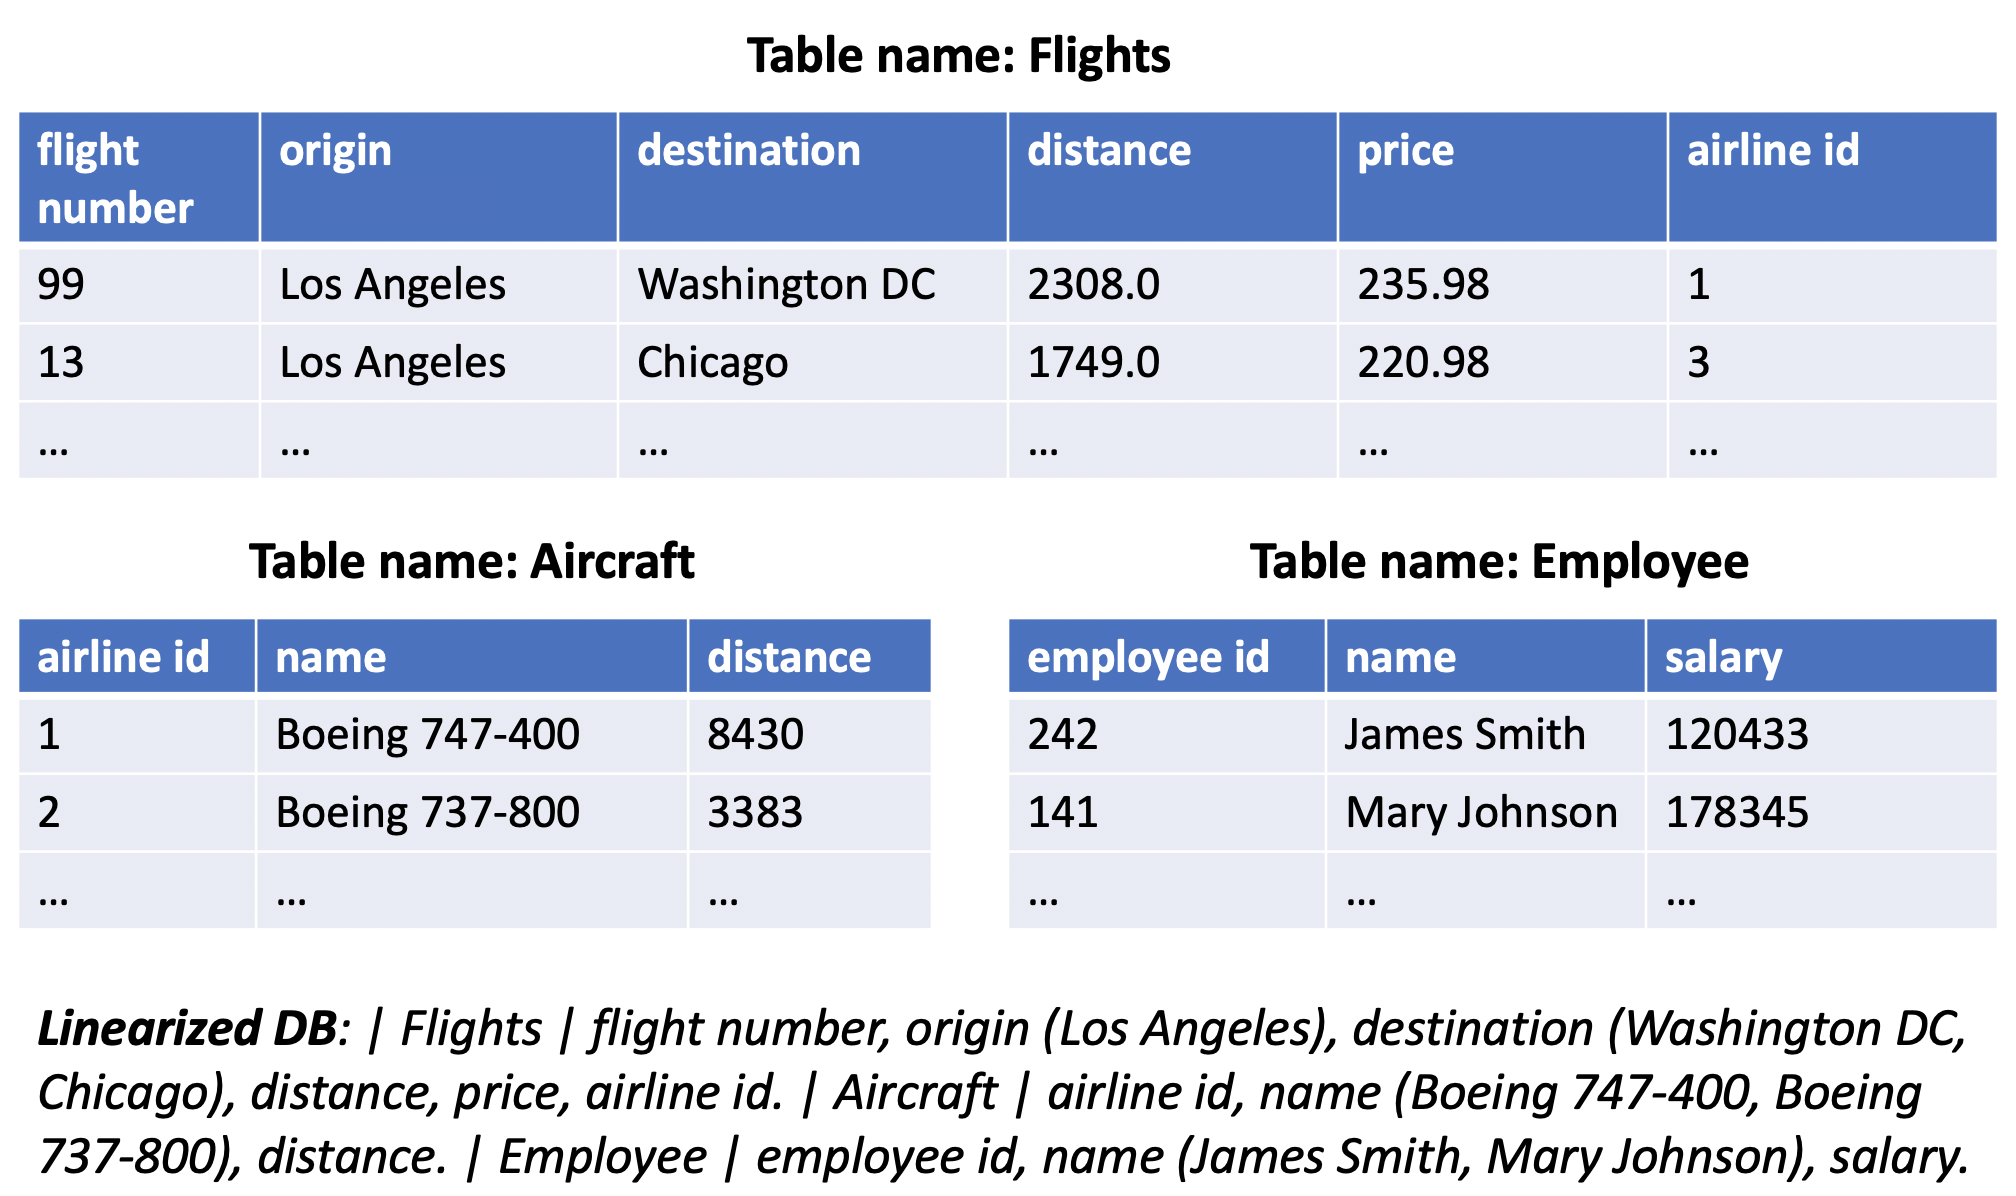
\includegraphics[width=0.8\linewidth]{figs/db-linearize.png}
% \caption{An example of DB linearization. Notice that the included cell values are deliberately selected to showcase the idea; in practice, cells are not always available, depending on the dataset, and cell value selection is non-trivial and method-specific.}
% \label{fig:db-linearize}
% \end{figure}



\begin{figure}[h]
\centering
\subfloat[DB linearization.]{\label{fig:db-linearize}{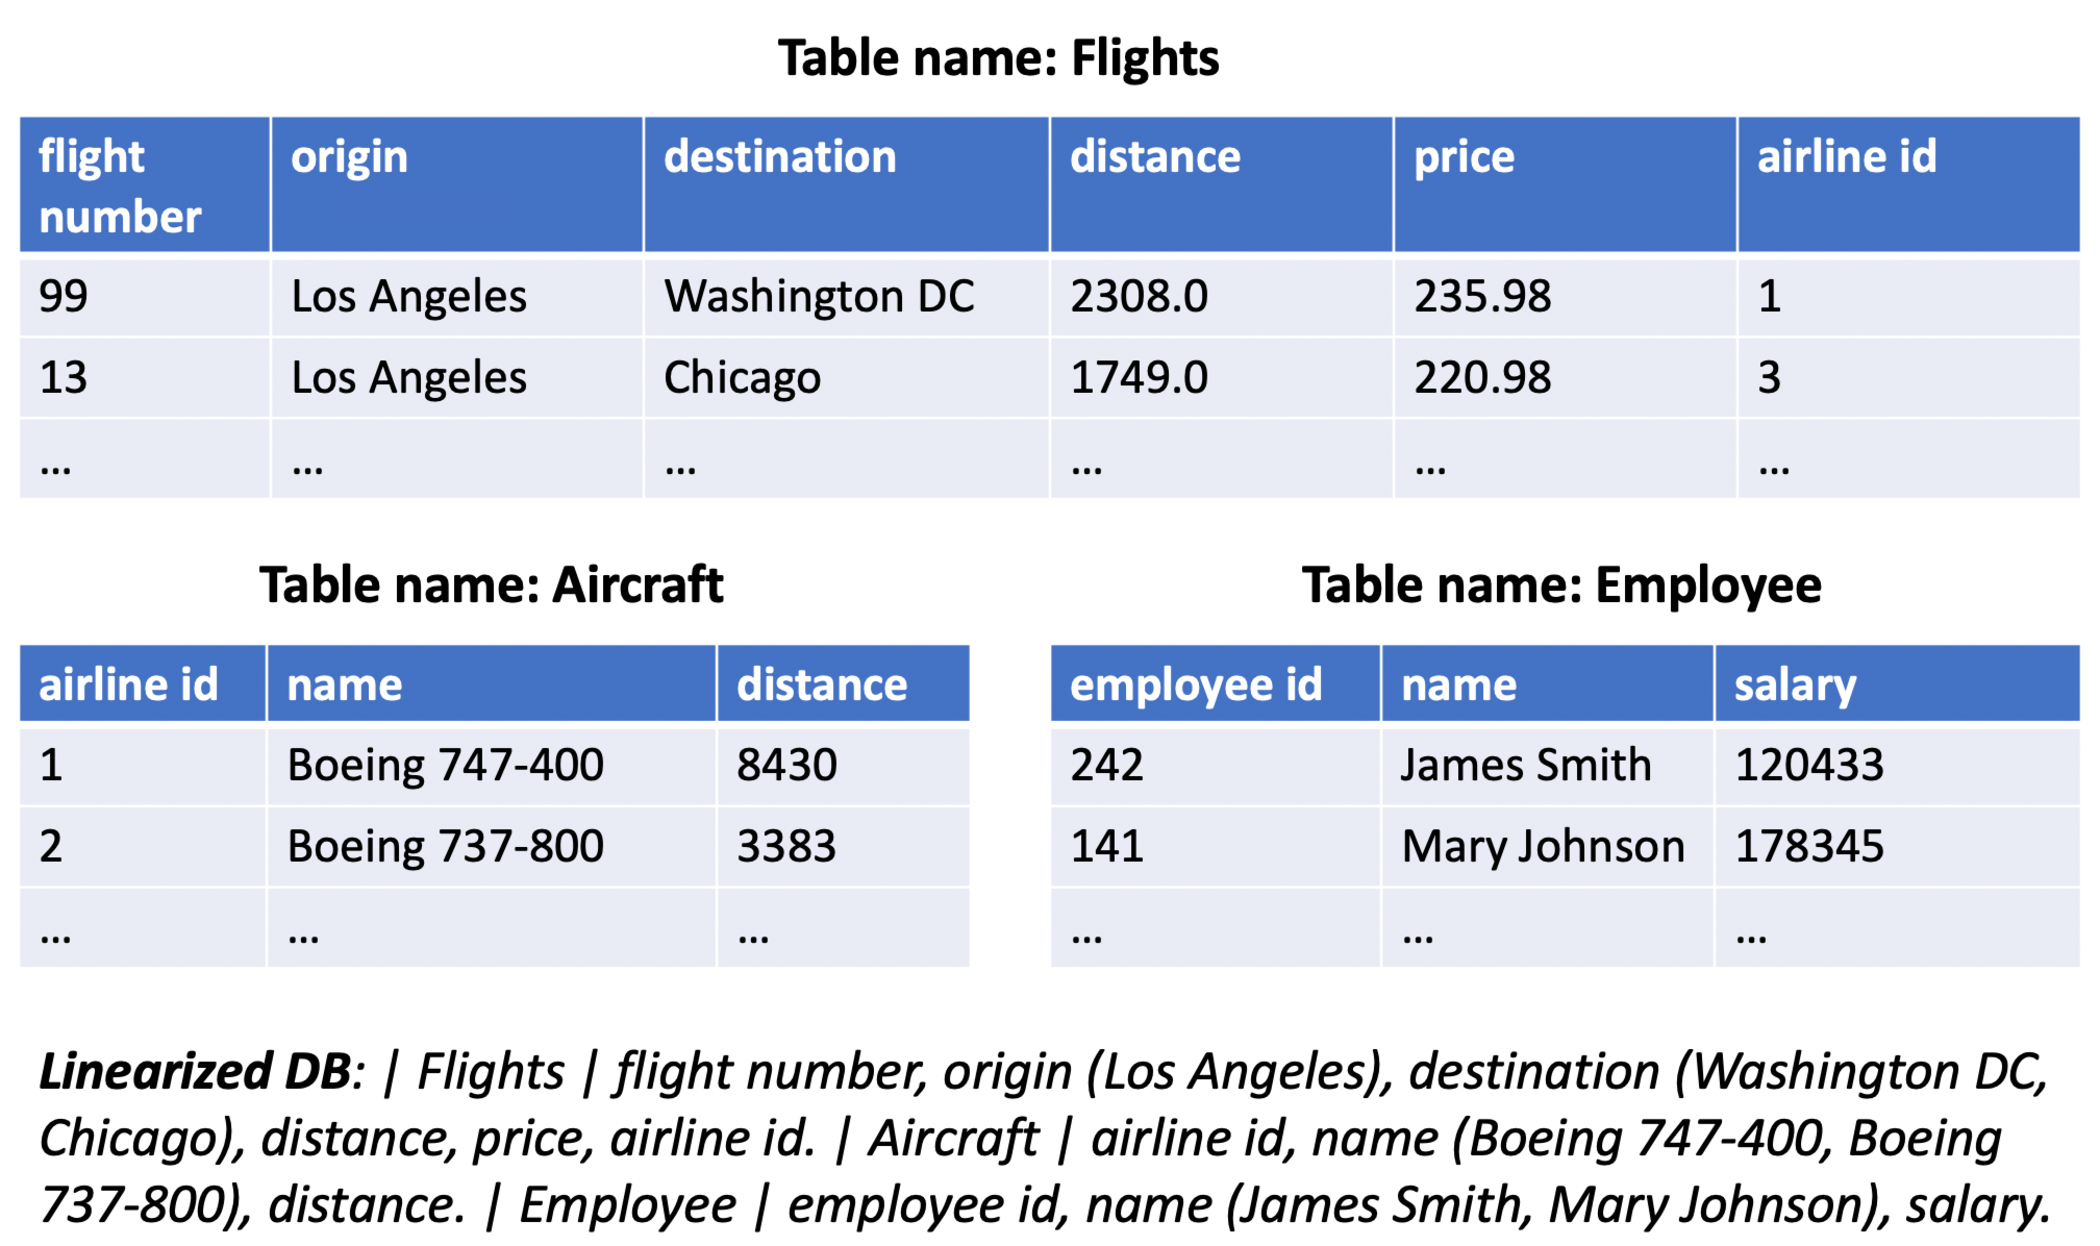
\includegraphics[width=0.55\linewidth]{figs/db-linearize.pdf}}}~
\subfloat[DB graph.]{\label{fig:db-graph}{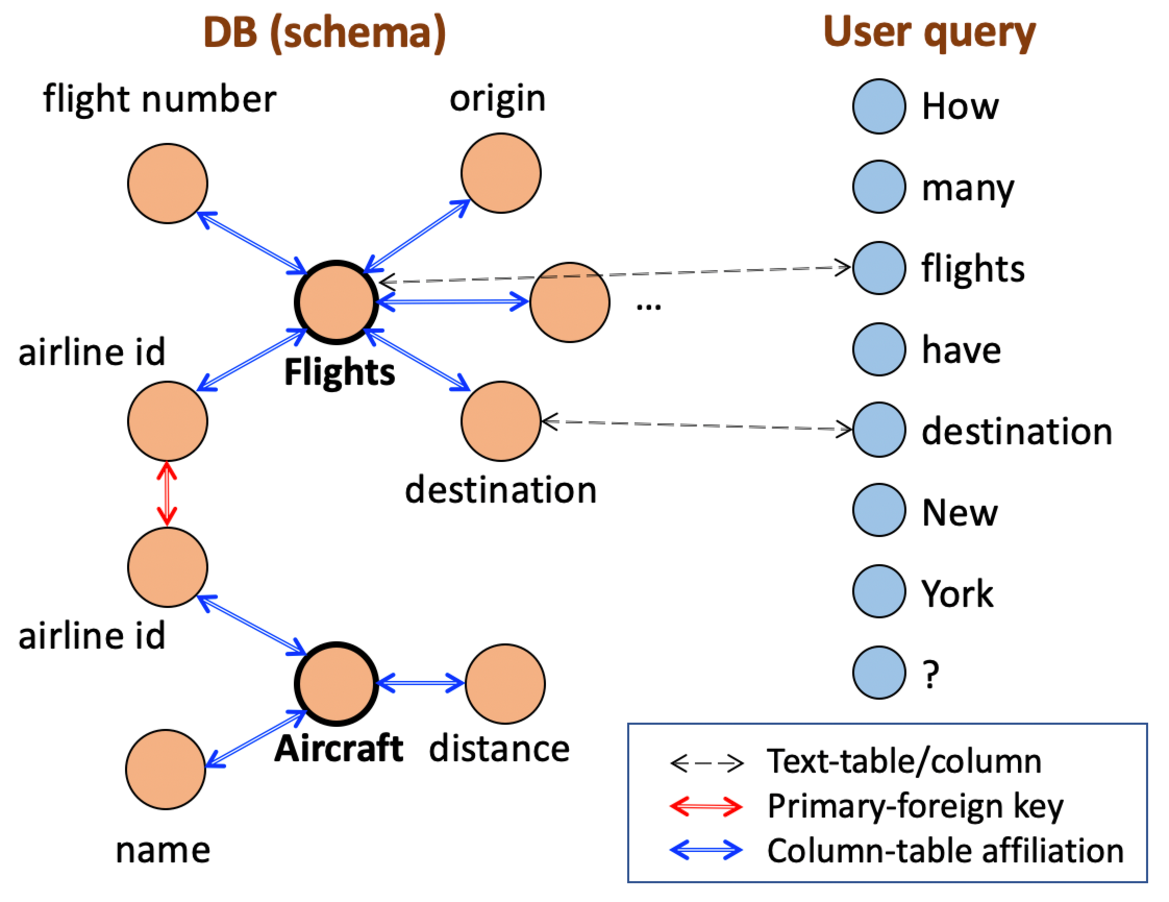
\includegraphics[width=0.4\linewidth]{figs/schema-text-graph.pdf}}}
% \vspace{0.2cm}
\caption{DB linearization and graph illustration. (a) An example of DB linearization. Notice that the included cell values are deliberately selected to showcase the idea; in practice, cells are not always available, depending on the dataset, and cell value selection is non-trivial and method-specific. (b) An example of DB graph. Some columns, tables and cells are omitted for visualization clarity. In detail, the design of relation set is also method-specific. This figure only illustrates the high-level idea.}
\label{fig:db-line-and-graph}
\end{figure}



\subsubsection{Table Representation}
Essentially, a DB is made up by tables; therefore, we can exploit the tabular structure to better represent the information.
% Many existing works 
A lot of exisiting work target table representation, not specific for text-to-SQL but generally for any task involving tables (other tasks include table QA, table-text entailment, etc.)~\cite{tapas,tableformer}.
% There are also works
Some approaches leverage properties of tables together with linearization. For example, \cite{tabert} first applies a \textit{horizontal transformer} to get text-row representations for rows in the table, then a \textit{vertical transformer} between all text-row representations to obtain a single text-table representation.

\subsubsection{Graph Representation}
There is another line of work to represent the table based on graph structure. We can define relations between question tokens and DB entities (e.g. table names, column names, cell values). Example relations include \textit{table-column affiliation} between tables and columns; \textit{primary-foreign key} between columns; \textit{token-table/column mention} between question tokens and tables or columns; etc. Such relations form a graph where each token / DB entity is a node, and each existing relation is an edge. An example of such graph is shown in Figure~\ref{fig:db-graph}. Given such a graph, we can use graph neural network to encode it~\cite{schema-gnn,lgesql}. We can also use the relations directly to enhance linearization-based methods. For example, we can add a \textit{relational bias} term in self-attention layers in transformers. Each relation has a learnable bias vector; when computing the attention weights between two tokens, if they exhibit a relation, we add the corresponding bias vector into the token representation~\cite{ratsql,s2sql} (similar ideas are also studied in table-only representation, such as in~\cite{tableformer}).

\subsection{Structured Data Representation in Speech-to-SQL}
We introduce our research on speech-to-SQL.\footnote{Under submission. We focus on the high-level ideas and omit the details in order not to violate submission policies.}
Most existing studies focus on text-to-SQL which is to parse natural language \textit{text} utterances into  executable SQL queries.
Motivated by the rise of speech-driven digital assistants on smartphones, tablets, and other small handheld devices, we study the task of parsing spoken natural language (in audio) to executable SQL queries (speech-to-SQL parsing). A speech-to-SQL parser has a number of potential use scenarios for quick and convenient data look-up, such as patient caring (in healthcare domain), business meeting, or driving.
% For example, in the healthcare domain, a nurse practitioner at a patient bedside typically looks up patient details on a desktop in the patient's room by filling out forms whose back-end is a database, where speech-to-SQL could  be used instead, for faster results.  
% Furthermore, speech-to-SQL removes the need  for keyboards that can be slow and cumbersome on small devices,  when querying databases.
In this work, we study ways to improve speech-to-SQL parsers. We will also highlight the representation of structured data, i.e. the DB, in this study.

\subsubsection{Baselines}
An obvious solution of speech-to-SQL parsing is to first pass the speech audio through an automatic speech recognizer (ASR), and then issue the top-ranked ASR transcription to a text-to-SQL parser which produces the final SQL.
%  This approach is depicted in Figure~\ref{fig:baselinevsproposed}.
We name it the \textit{blackbox} baseline.
A drawback of this baseline is that no attempt is made to deal with ASR errors. Figure~\ref{fig:speakql-figure-1}(A) shows an example of such errors. Passing ASR errors to the text-to-SQL parser is unlikely to produce the correct SQL.

For ASR error correction, we import two more baselines from previous work: \textit{re-ranker} and \textit{S2S-rewriter} baseline. The re-ranker takes the top-K candidate transcriptions from ASR and re-rank them to select the best transcription~\cite{ASR-Reranker}. In contrast, the S2S-rewriter directly rewrites an ASR transcription into a better sentence, as a S2S task~\cite{ASR-S2S}. Both methods do not incorporate the DB information.

\subsubsection{Method Overview}
We propose a two-stage ASR error correction method. First, we \textit{tag} the input sentence (an ASR transcription) to identify tokens that are incorrect and should be edited. Second, we edit the sentence using a \textit{blank-filling} model, where the tagged incorrect parts of the sentence are regarded as blanks and filled by predicted tokens.
Moreover, we incorporate the backend DB information into the model by adding the DB schema and relevant cell values into the input sentence, in the above-mentioned \textit{linearized} manner. Figure~\ref{fig:speakql-figure-1} illustrates the framework of our method.
% It falls under the category of rewriter, as the method is able to freely edit the transcription text.

\begin{figure}[h]
\centering
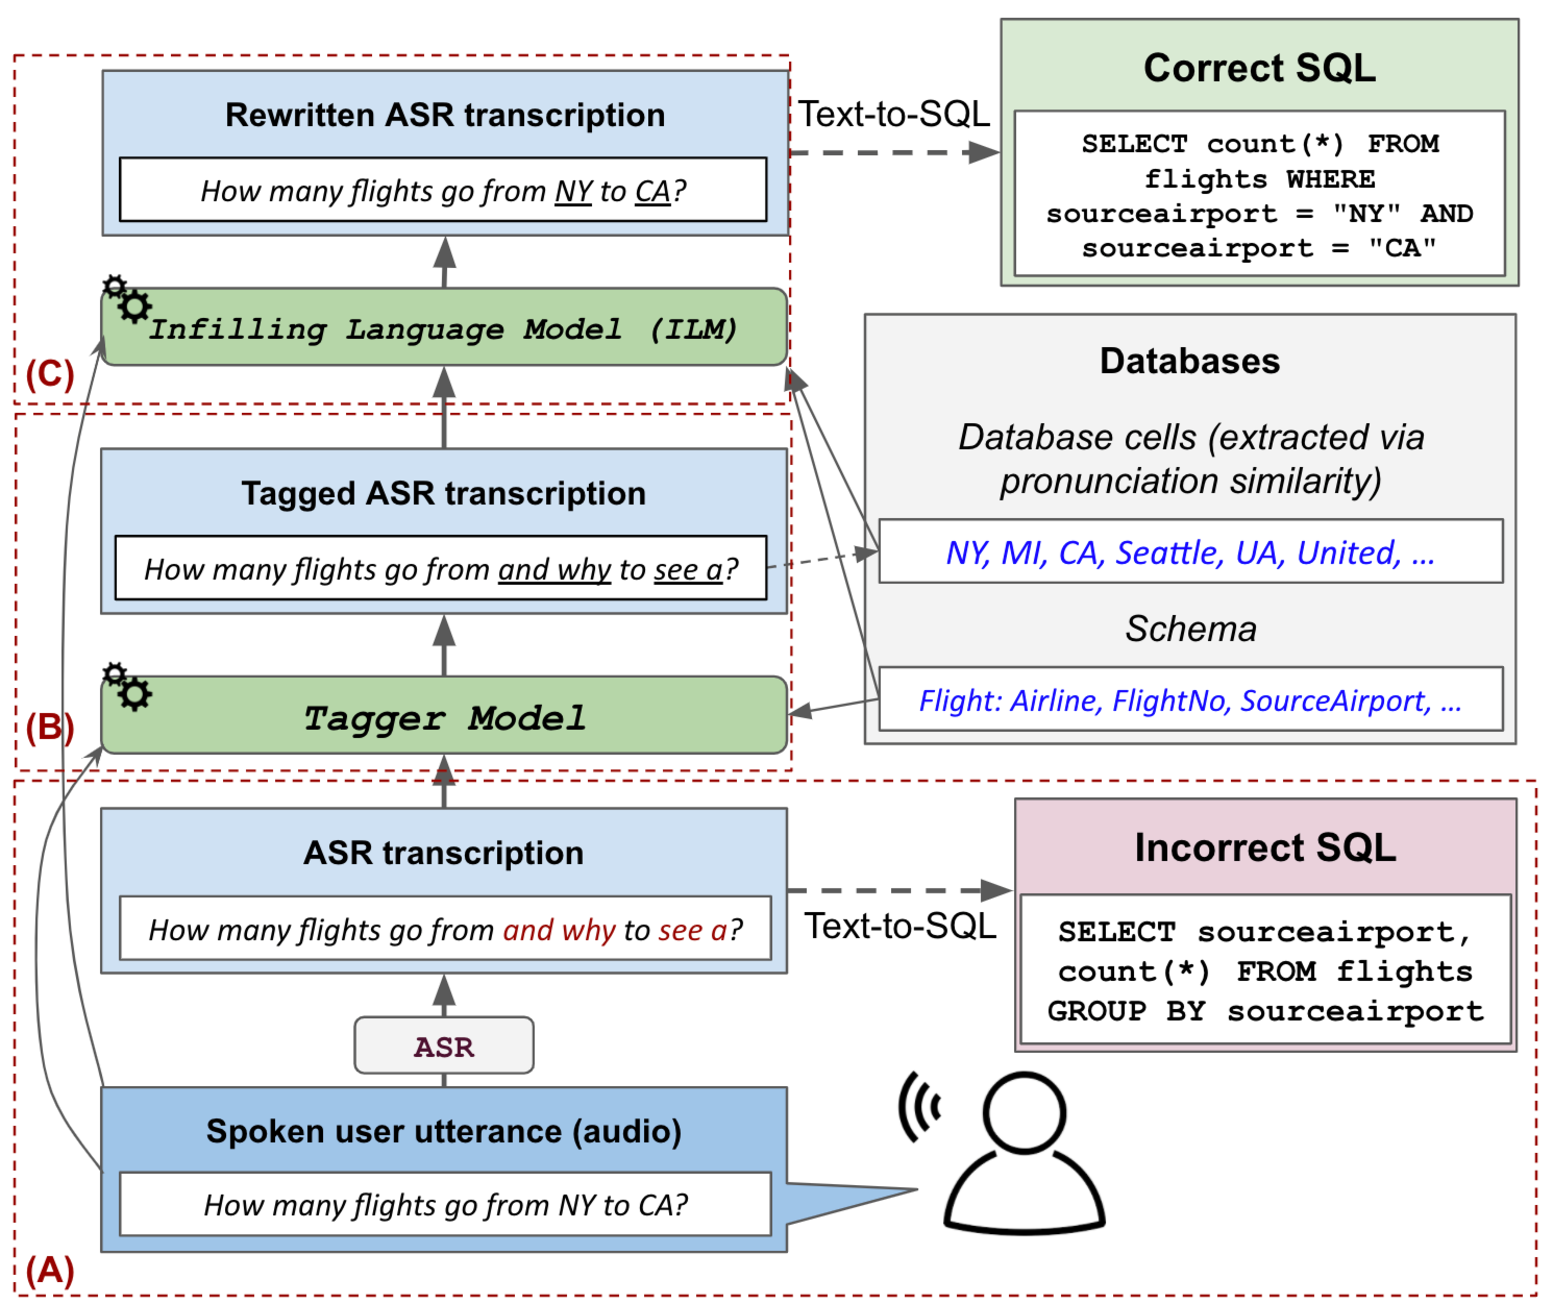
\includegraphics[width=0.7\linewidth]{figs/speakql-fig1.pdf}
\caption{Overview of the ASR correction method for speech-to-SQL. (A) Directly passing the erroneous ASR transcription to text-to-SQL parser will likely produce wrong SQL output. We apply a Tagger (B) and an ILM (blank-filling) rewriter (C) to fix the transcription, incorporating audio features and DB information.}
\label{fig:speakql-figure-1}
\end{figure}


\subsubsection{Experiments and Analysis}
\paragraph{Datasets} Experiments are conducted on the Spider dataset mentioned above. To make it usable for evaluation speech-to-SQL methods, we used Amazon Polly, a text-to-speech (TTS) service, to automatically transform the user queries from text to audio. We used Amazon Transcribe as the raw ASR transcriber.
Besides, since our method focuses on ASR correction, we utilize existing models as the backend text-to-SQL parser during evaluation. We use RAT-SQL~\cite{ratsql} and T5 (T5-base and T5-large)~\cite{uskg}, which are representative and competitive text-to-SQL parsers.

\paragraph{Evaluation Metrics} We test baseline methods and our proposed methods on two categories of metrics. The first category is on \textit{text accuracy}, for which we use \textit{word error rate (WER)} and \textit{BLEU score}. The second category measures the final \textit{SQL accuracy}, for which we use \textit{exact match rate} and \textit{execution match rate} of the SQL predictions against ground truth.

\paragraph{Results}  We test and compare our proposed methods to all baseline methods (blackbox, re-ranker, S2S-rewriter) on Spoken Spider.
Results show that our proposed method can outperform all baseline methods on both category of metrics, regardless of backend parser. We also conducted ablation studies to profile the source of performance gain. The results show that the tagging + blank-filling pipeline, compared to re-ranker or S2S-rewriter, is the major source of improvement. Nonetheless, the incorporation of structured data, i.e. DB information, also provides non-negligible benefits. We would also like to highlight that, retrieving and adding relevant cells into the input can substantially improve the performance, compared to only using the DB schema.


\section{Task-oriented Dialog Systems}

\subsection{Real Application Example}
As mentioned, a TOD system can help users complete actions more easily, especially in complex scenarios where multi-turn interactions are needed.
One of the real use cases is on \textit{data plotting}.
Plotting is a very common practice for visualizing data and mathematical functions.
Existing plotting libraries such as  \texttt{matplotlib} support a decent range of functionalities. However, using such libraries can be difficult for novice users and time consuming even for experts, due to both the hardness of programming and complexity of our detailed plotting needs.
It thus motivates us to build a TOD system that helps human complete plotting tasks by interacting with users through natural language.

In what follows, we first provide a more general and formal introduction to the TOD systems. We then survey related work in this direction, and introduce our own work on the above-mentioned plotting task.

\subsection{Formal Introduction}
% As mentioned, a TOD system helps users to complete actions. 
A TOD system runs in one or several \textit{domains} and requires a domain-specific \textit{ontology}. Intuitively, an ontology is a set of slots and values for each slot, representing the domain-specific information required by the system or the user.
% Many existing datasets split slots into \textit{informable} and \textit{requestable} ones: \textit{informable} slots are provided by the user and used by the system to search in the backend; \textit{requestable} slots can requested by the user and are provided by the system based on its searching results \cite{DSTC2,multiwoz}.
Several example ontologies are shown in Figure~\ref{fig:sample-onto}.


\begin{figure}[h]
\centering
    \subfloat[The ontology of MultiWOZ~\cite{multiwoz}. For each slot, the upperscript indicates the domain indexes it belongs to. *: universal, 1: restaurant, 2: hotel, 3: attraction, 4: taxi, 5: train, 6: hospital, 7: police.]{
    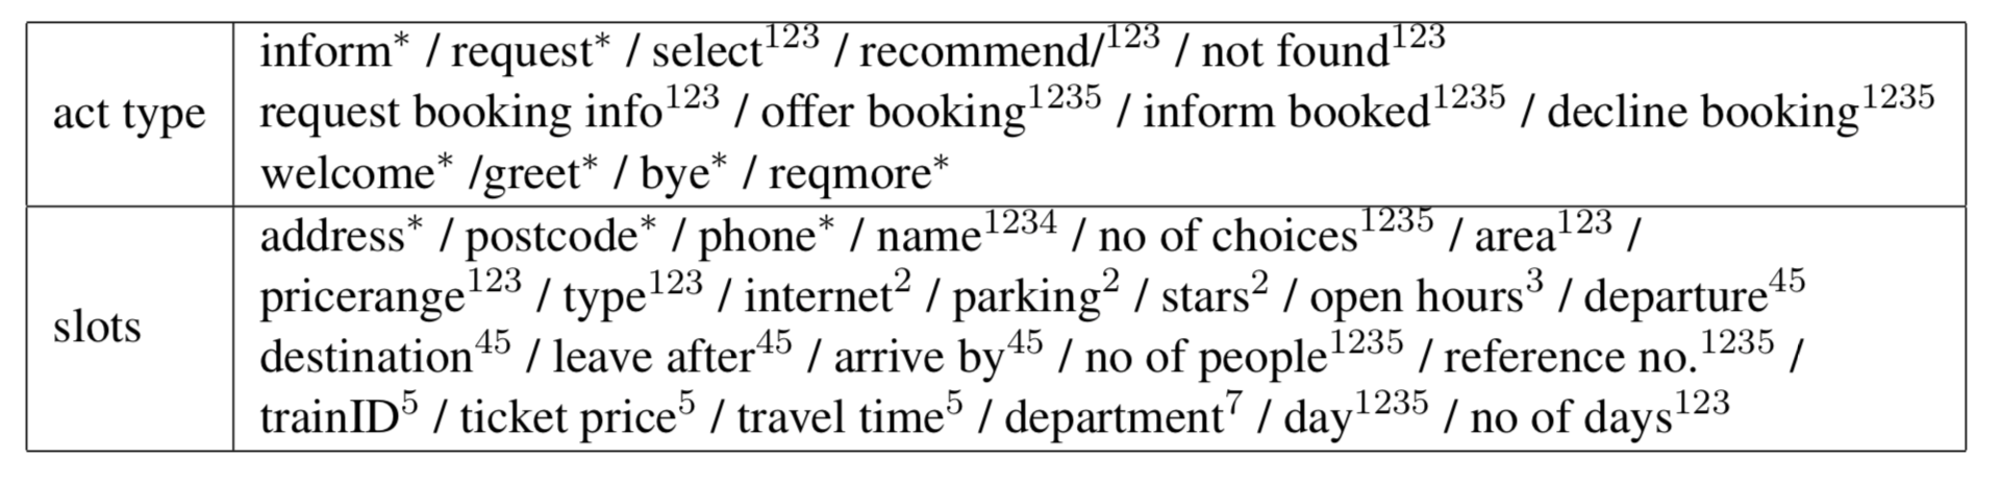
\includegraphics[width=0.6\linewidth]{figs/MultiWOZ-onto.pdf}
    \label{fig:MultiWOZ-onto}}~\hspace{0.4cm}
    \subfloat[The ontology of DSTC2~\cite{DSTC2}. The domain is restaurant booking.]{
    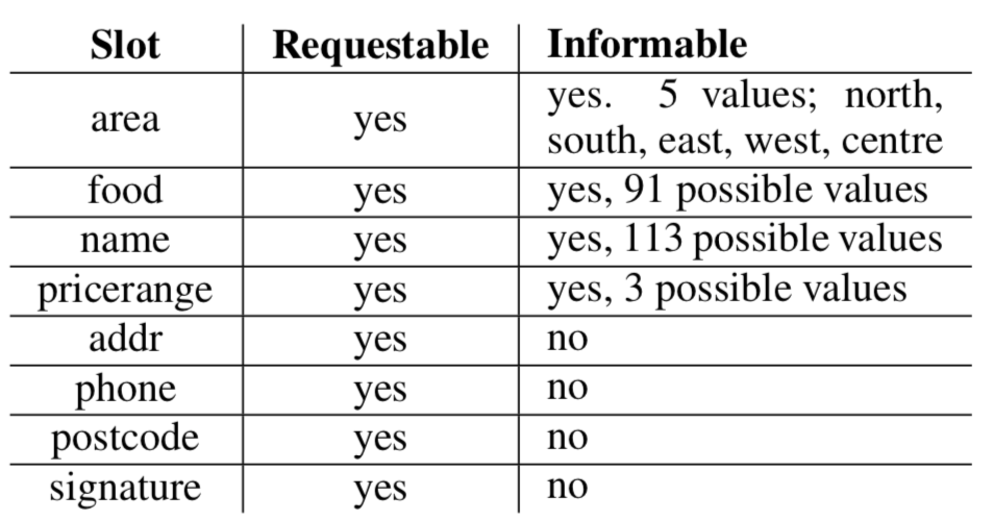
\includegraphics[width=0.3\linewidth]{figs/DSTC2-onto.pdf}
    \label{fig:DSTC2-onto}}
\caption{Sample ontology of existing datasets.}
\label{fig:sample-onto}
\end{figure}


There are two main categories of TOD system design: pipeline-based and end-to-end \cite{Zhang2020RecentAA}. A pipeline-based TOD system consists of a collection of separate modules, including natural language understanding (NLU), dialog state tracking (DST), dialog policy, and natural language generation (NLG).
In contrast, an end-to-end TOD system directly takes the current user utterance and dialog history as input, and predicts the action or response.
% Most of recent neural models for task-oriented dialog are built in an end-to-end manner. However, they may add modules or designs in the neural model referring to the steps in the pipeline, in order to improve performance.

% As an early work in the thread of end-to-end task-oriented dialog systems, \cite{bAbIDialog} built a dataset called bAbI dialogs which involves a real task of restaurant booking. The bAbI dialog dataset was generated by template filling, therefore can be perfectly solved by a rule-based system. They tested the performance of several kinds of end-to-end neural models on this dataset.

Structured data in TOD systems is a complex topic, because a TOD system involves several different types of structured data, mainly including two categories: \textit{internal} and \textit{external} structured data.
External structured data include the backend DB or KG, similar to the structured data for semantic parsing as mentioned above. 
Internal structured data include \textit{dialog state} and \textit{dialog act}.
Dialog state is the output of the dialog state tracking component.
It includes the user intents and specified values for each slot. It can be transformed into a DB query to search for relevant information, which may also be used by the model to decide the response.
Dialog act is the output of dialog policy component. It controls what the system response wants to achieve. Basically, for system response generation we care about ``what to say'' and ``how to say it''; the dialog act is the ``what to say'' part.
% (See Figure~\ref{fig:babi-sample} for examples of dialog states and dialog acts)



% Among the ``subtasks'' of task-oriented dialog systems, the \textit{dialog state tracking (DST)}, also known as \textit{belief tracking}, is arguably the most important subtask. It aims to predict and update the \textit{dialog state} after each user utterance. The dialog state includes the user intents and specified values for each slot (see Figure~\ref{} for examples of dialog states). Many end-to-end methods have explicit modeling for dialog state tracking, such as \cite{}.
% % It can be regarded as a special form of frame-semantic parsing where a frame corresponds to a user intent, and an argument or semantic role corresponds to a slot.
% Dialog state tracking can be regarded as a form of semantic parsing, where the logical form is the dialog state, i.e. intent and slot-value pairs.
% The dialog states are structured data; they are essentially a sub-table (with 1 row) based on the domain ontology.
% % Thus, besides interacting with the external structured data (DB or KG), the dialog model would also need to predict, update and leverage such ``internal'' structured data throughout the dialog process.
% Thus, besides handling ``external'' structured data (DB or KG), the dialog model would also need to predict, update and leverage such ``internal'' structured data throughout the dialog process.

\subsection{Structured Data Representation in Task-oriented Dialog Systems}
% As mentioned, different from semantic parsing which focuses on handling external structured data for the sake of generalizing across domains, the task-oriented dialog systems mostly focus on a single domain, thus the major focus is on the internal structured data, i.e. the dialog state.
% In the section of semantic parsing we have discussed a lot of methods to represent external structured data, i.e. DB or KG. For task-oriented dialog system, we focus more on the internal structured data, i.e. dialog state.

% In the section of semantic parsing we have discussed a lot of methods to represent external structured data, i.e. DB or KG. For task-oriented dialog system, we focus more on the internal structured data, i.e. dialog state.

\subsubsection{External}
\paragraph{Database (DB)}
In TOD systems, we utilize the backend DB by queries based on the dialog state (the user-specified slot values are conditions in the query). How the DB query results are utilized depends on the task setting, or practically, the dataset.
On certain datasets, the systems are required to use the full content. For example, in the bAbI dialog dataset~\cite{bAbIDialog}, given all the records satisfying user-specified conditions, the system is expected to ``learn'' to rank results by the field named ``rating''. In such scenarios, the system usually regard the records as sentences in the dialog history.
On the other hand, many datasets do not have the explicit requirement~\cite{DSTC2,multiwoz,wen2017EndtoEnd}. As a result, a widely adopted heuristic is to simply use the \textit{number of records} in the query results, instead of the full results content~\cite{wen2017EndtoEnd,liu2018DialogueHumanTeaching,zhang2020LatentBeliefState}. The input and output of the model may be \textit{delexicalized}, i.e. using placeholders for entities (e.g. \texttt{[v.HOTEL\_NAME]} for a hotel name), which are replaced by actual entities in the query results during post-processing. In this way, in the dialog model, the query results are no longer structured data, but a single token (representing the number) that can be simply represented using look-up embeddings.


\paragraph{Knowledge Graph (KG)}
Knowledge graphs (KG) are frequently used in the task of \textit{knowledge-grounded dialogs}, in which the user chats with the dialog system to ask questions, learn knowledge or gather information, and the system responses based on external knowledge. This task does not rigorously belong to the definition of TOD, since the system does not make explicit backend API calls. Nonetheless, this task is highly related to TOD in the sense of retrieving relevant information from external data.
One way to represent KG is to simply use the (subj, rel, obj) triplet form. For example, in methods based on memory networks~\cite{mem2seq,wmm2seq}, each triplet in the KG are vector-embedded and added to the memory bank. During response generation, the token prediction probability includes a term to copy tokens from the KG triplets.
% ; when copying, copy the object.
Another line of work leverages the graph-structure of KG by ``walking'' on the edges, simulating human reasoning.
These methods can use the encoding vector of current turn information as the initial state.
They may iteratively update the state using a gated recurrent cell, each step attending to all walkable nodes \cite{moon2019OpenDialKG}, or directly predict a sequence of relations to decide the walking path \cite{cohen2020ScalableNeural,tuan2022TowardsLI}.
% \cite{tuan2022TowardsLI} use dialog history encoding vector to walk on KG. Use 3 heads to predict logical operation vector on current state, walking next state vector (next node, but soft), and decision vector to choosing (gating) between the two.


\subsubsection{Internal}

As mentioned, internal structured data in TOD systems mainly include dialog state and dialog act. Some fully end-to-end models do not have explicit modeling for internal structured data~\cite{mem2seq,wmm2seq}. However, it decreases the transparency, interpretability and controllability of the model. Thus, despite of the competitive performance of such models, it is still beneficial to explicitly predict and incorporate the internal structured data. Here we put more attention on incorporation and less on prediction. On prediction side, dialog state tracking and dialog policy learning are both popular research topics and involve a large variety of task-specific methods, which are out of the scope here.

\paragraph{Linearization}
A straightforward yet useful way to represent internal structured data is \textit{linearization}, similar to above-mentioned DB linearization in semantic parsing. We represent the dialog state and/or dialog act as token sequences, and encode them as text.
This type of method can be used for both prediction and incorporation, creating a unified pipeline for end-to-end dialog model where the ``internal states'' are always text.
For example, in~\cite{sequicity}, the dialog model is formulated as a two-stage sequence-to-sequence (S2S) model. First, based on previous dialog state and dialog history, predict current dialog state (this step is essentially dialog state tracking); second, based on dialog history and current dialog state, generate the response.
\cite{ham2020-gpt2-tod} considers TOD as a language modeling (LM) task by concatenating dialog history, dialog state, dialog act and response all together as a token sequence. They fine-tune a pretrained LM, GPT2, to predict dialog state, dialog act and response based on the input dialog history.

\paragraph{Other Specific Methods}
There are methods exploiting the determined structures of such internal structured data in order to effectively model them. For example, \cite{wen2017EndtoEnd} assumes a fixed domain and ontology, thus dialog state can be treated simply as a probability distribution per slot.
\cite{chen2019SemanticallyConditioned} exploits the (intent, slot, value) triplet structure of dialog act to build 3-layer tree to predict and control the encoder of dialog act.
% \cite{zhang2020LatentBeliefState} treats dialog state as latent variable, using variational learning.
Such methods can potentially have simpler design or have better performances on specific datasets; however, it is harder for them to generalize to other datasets or domains.


\subsection{Structured Data Representation in a Plotting Agent}
We introduce our original work on the novel task of \textit{plotting agent}, by which we refer to the above-mentioned TOD system for data plotting ~\cite{chartdialogs}.
% Plotting is a method for visualizing data and mathematical functions.
% Plotting libraries such as  \texttt{matplotlib} support  functionality on a range of levels,  from   general,  ``change the X-axis from $linear$ to $log$ scale'',  to specific,  ``color this screen pixel red''. Yet, using such libraries can be difficult for novice users and time consuming even for experts.
% This obstacle motivates our objective of designing  natural language interfaces~(NLIs) for plotting, which we name as a \textit{plotting agent}.
Notice that this plotting agent is targeted at manipulating the plot appearance (colors, shapes, sizes, etc.) instead of the underlying data.
% With a plotting agent, the user specifies how they would like to  manipulate a plot. As an example, consider the following questions from a community question answering forum for matplotlib \footnote{https://stackoverflow.com/questions/tagged/matplotlib}: ...
% Expressing these intents in natural language is often faster than perusing the documentation of plotting library, thus motivating the design of such plotting agents.
In this work, we collected a large-scale dataset for training a plotting agent, and conducted experiments on competitive methods to compare and analyse their performances. We also showcase the influence of structured data representations on model performances.

\subsubsection{Problem Definition}
We aim to develop a \textit{conversational plotting agent} that takes natural language instructions and updates the plot accordingly. The agent is designed conversational because plots can be complex, making it difficult to describe everything at once; thus, users may want to tune the appearance of their plot through multiple turns.
Technically, a conversational plotting agent is framed as a TOD system. It has only one domain, which is plot control. We manually defined the domain ontology to include several plot types and a large number of slots, based on \texttt{matplotlib} documentation and the common needs based on our experiences.
Figure \ref{fig:slotsfortwo} illustrates example slots for some of the plot types. The full ontology is shown in Table~\ref{tbl:chartdialogs-onto}.
Different plot types have different sets of slots, yet some slots are shared across plot types. % such as slots that are relevant for the axes.
For example, the  slot ``X-axis scale" is relevant to the X-axis, thus it is applicable in any plot type with an X-axis, including line chart, bar plot, contour plot, etc. For modeling purposes, the plot type can also be seen as a slot in the ontology.
Notice that, in the current definition, a conversational plotting agent is simpler than a ``full'' TOD system, because the system directly uses dialog states as responses and does not have to generate text responses.\footnote{We wrote a simple script that can take as input the dialog state (plot type and other slot values), to generate the actual plot image using \texttt{matplotlib} and display it to the user. Thus, plot controlling is equivalent to dialog state tracking.}



\begin{figure}[t]
\centering
\subfloat[Line Chart]{
    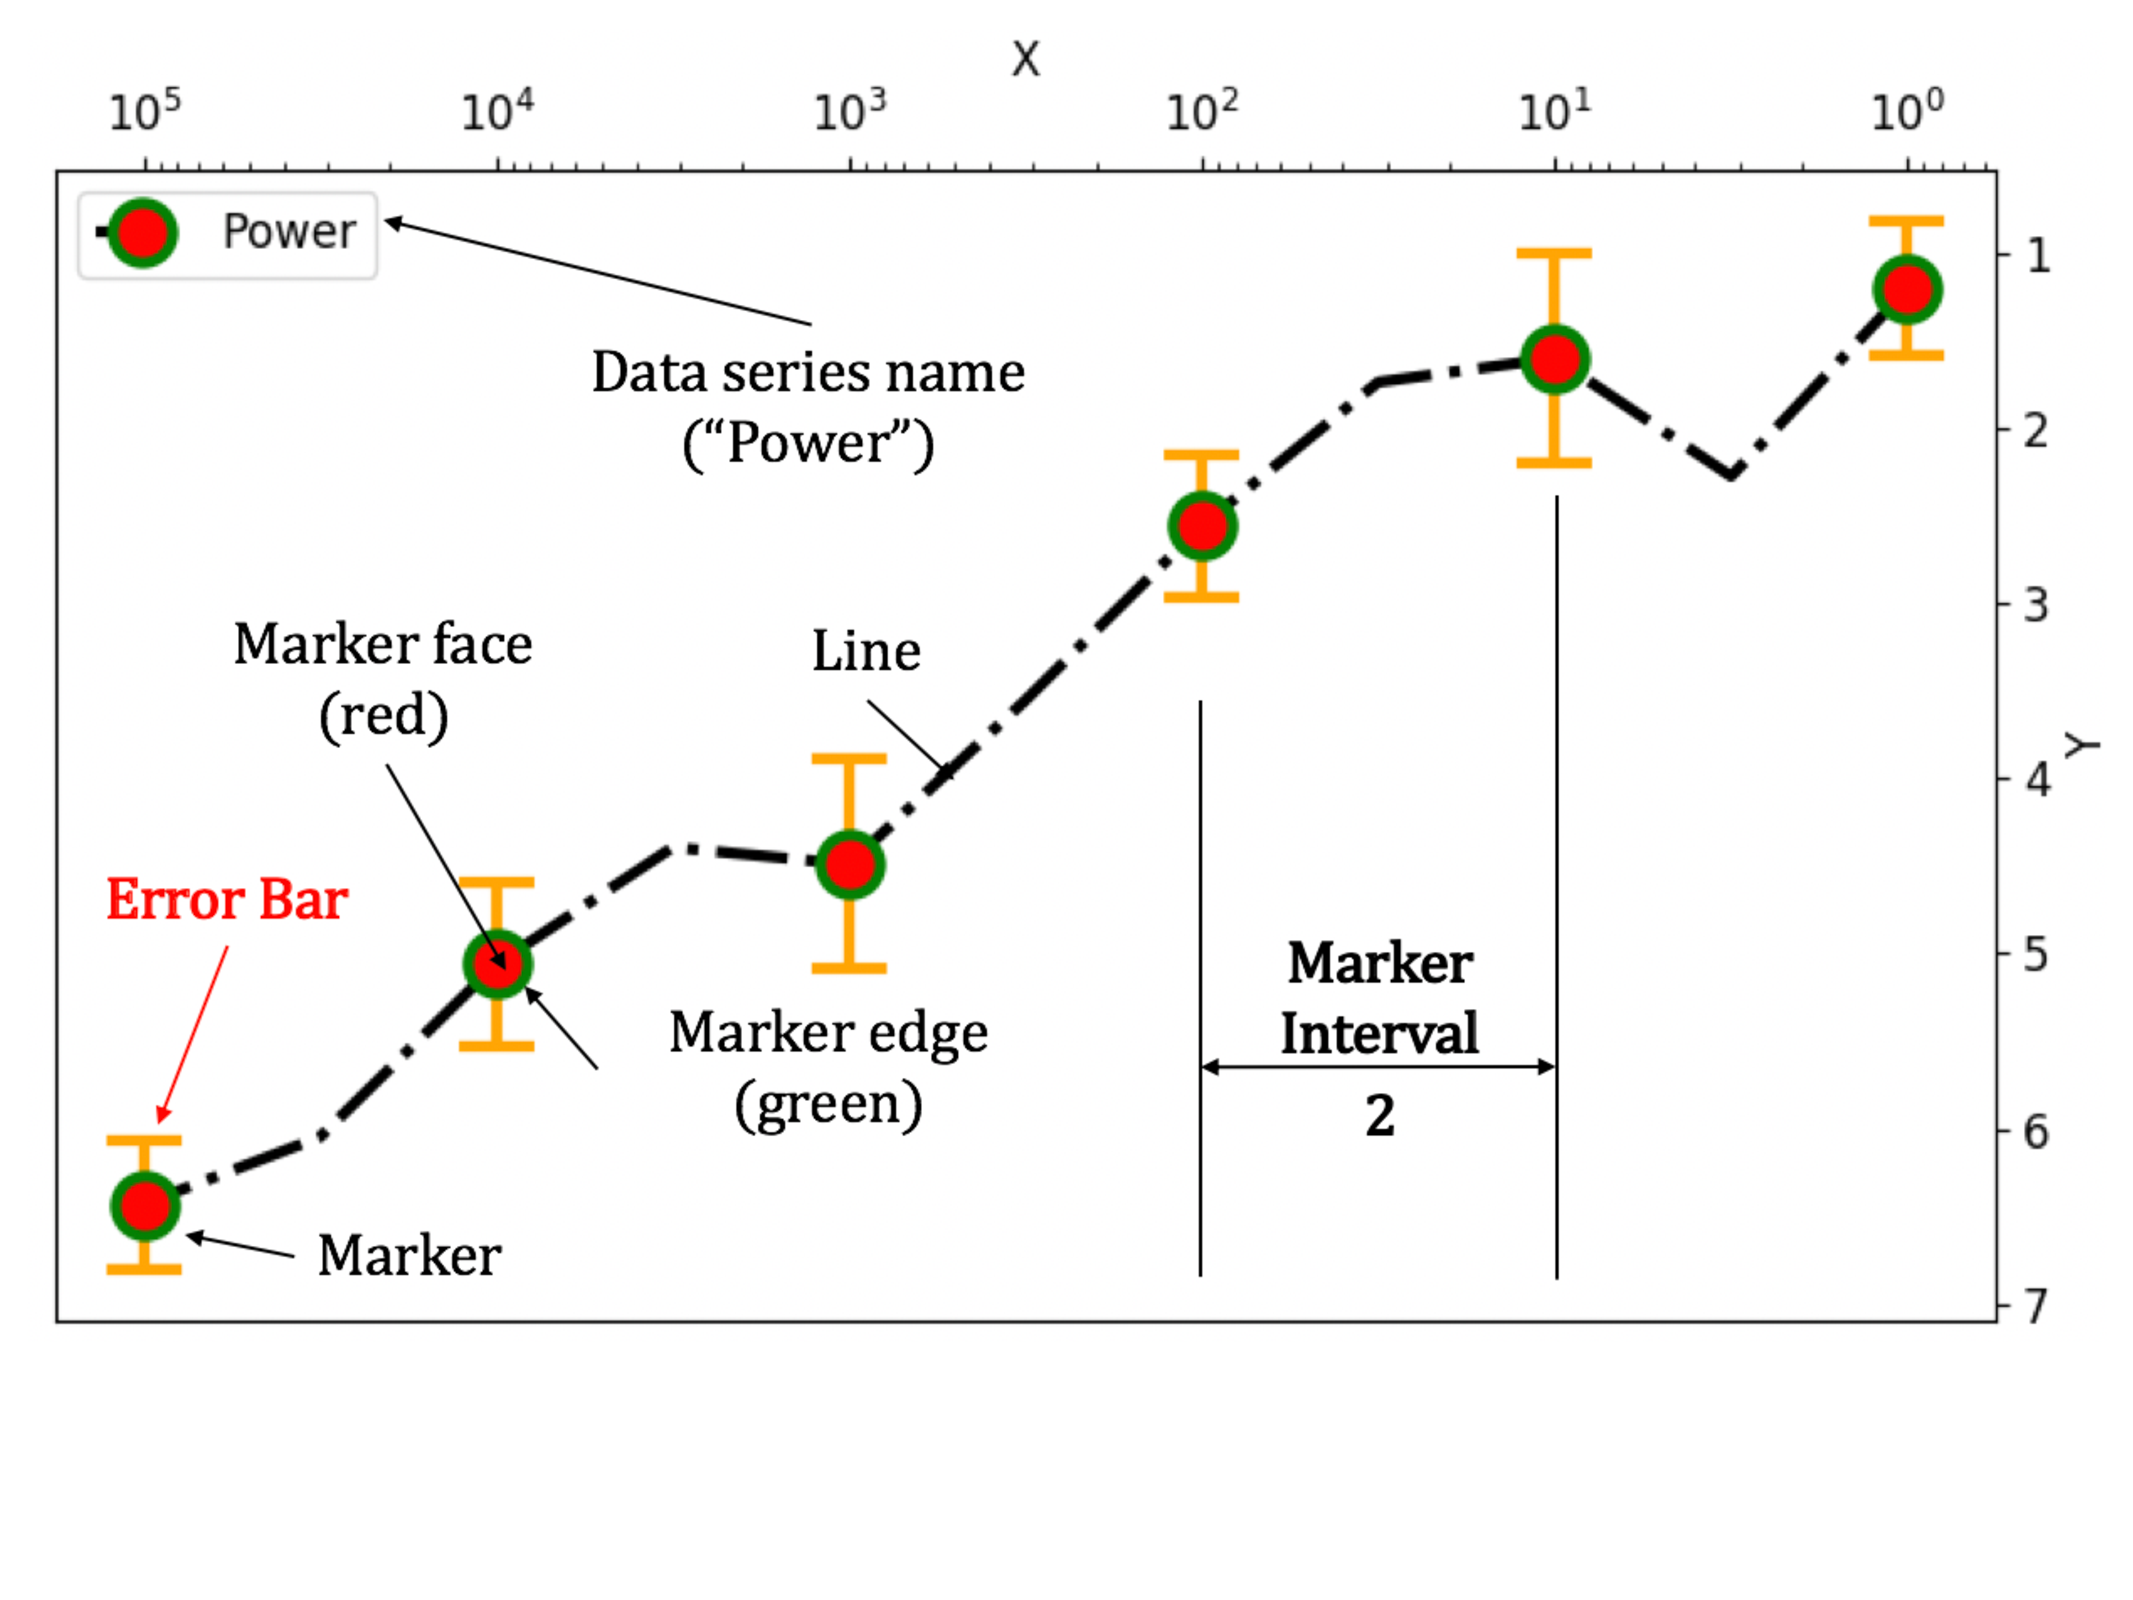
\includegraphics[width=0.45\linewidth]{figs/il-full-line.pdf}
    % \vspace{-0.8cm}
    \label{fig:line}}~
\subfloat[3D surface]{
    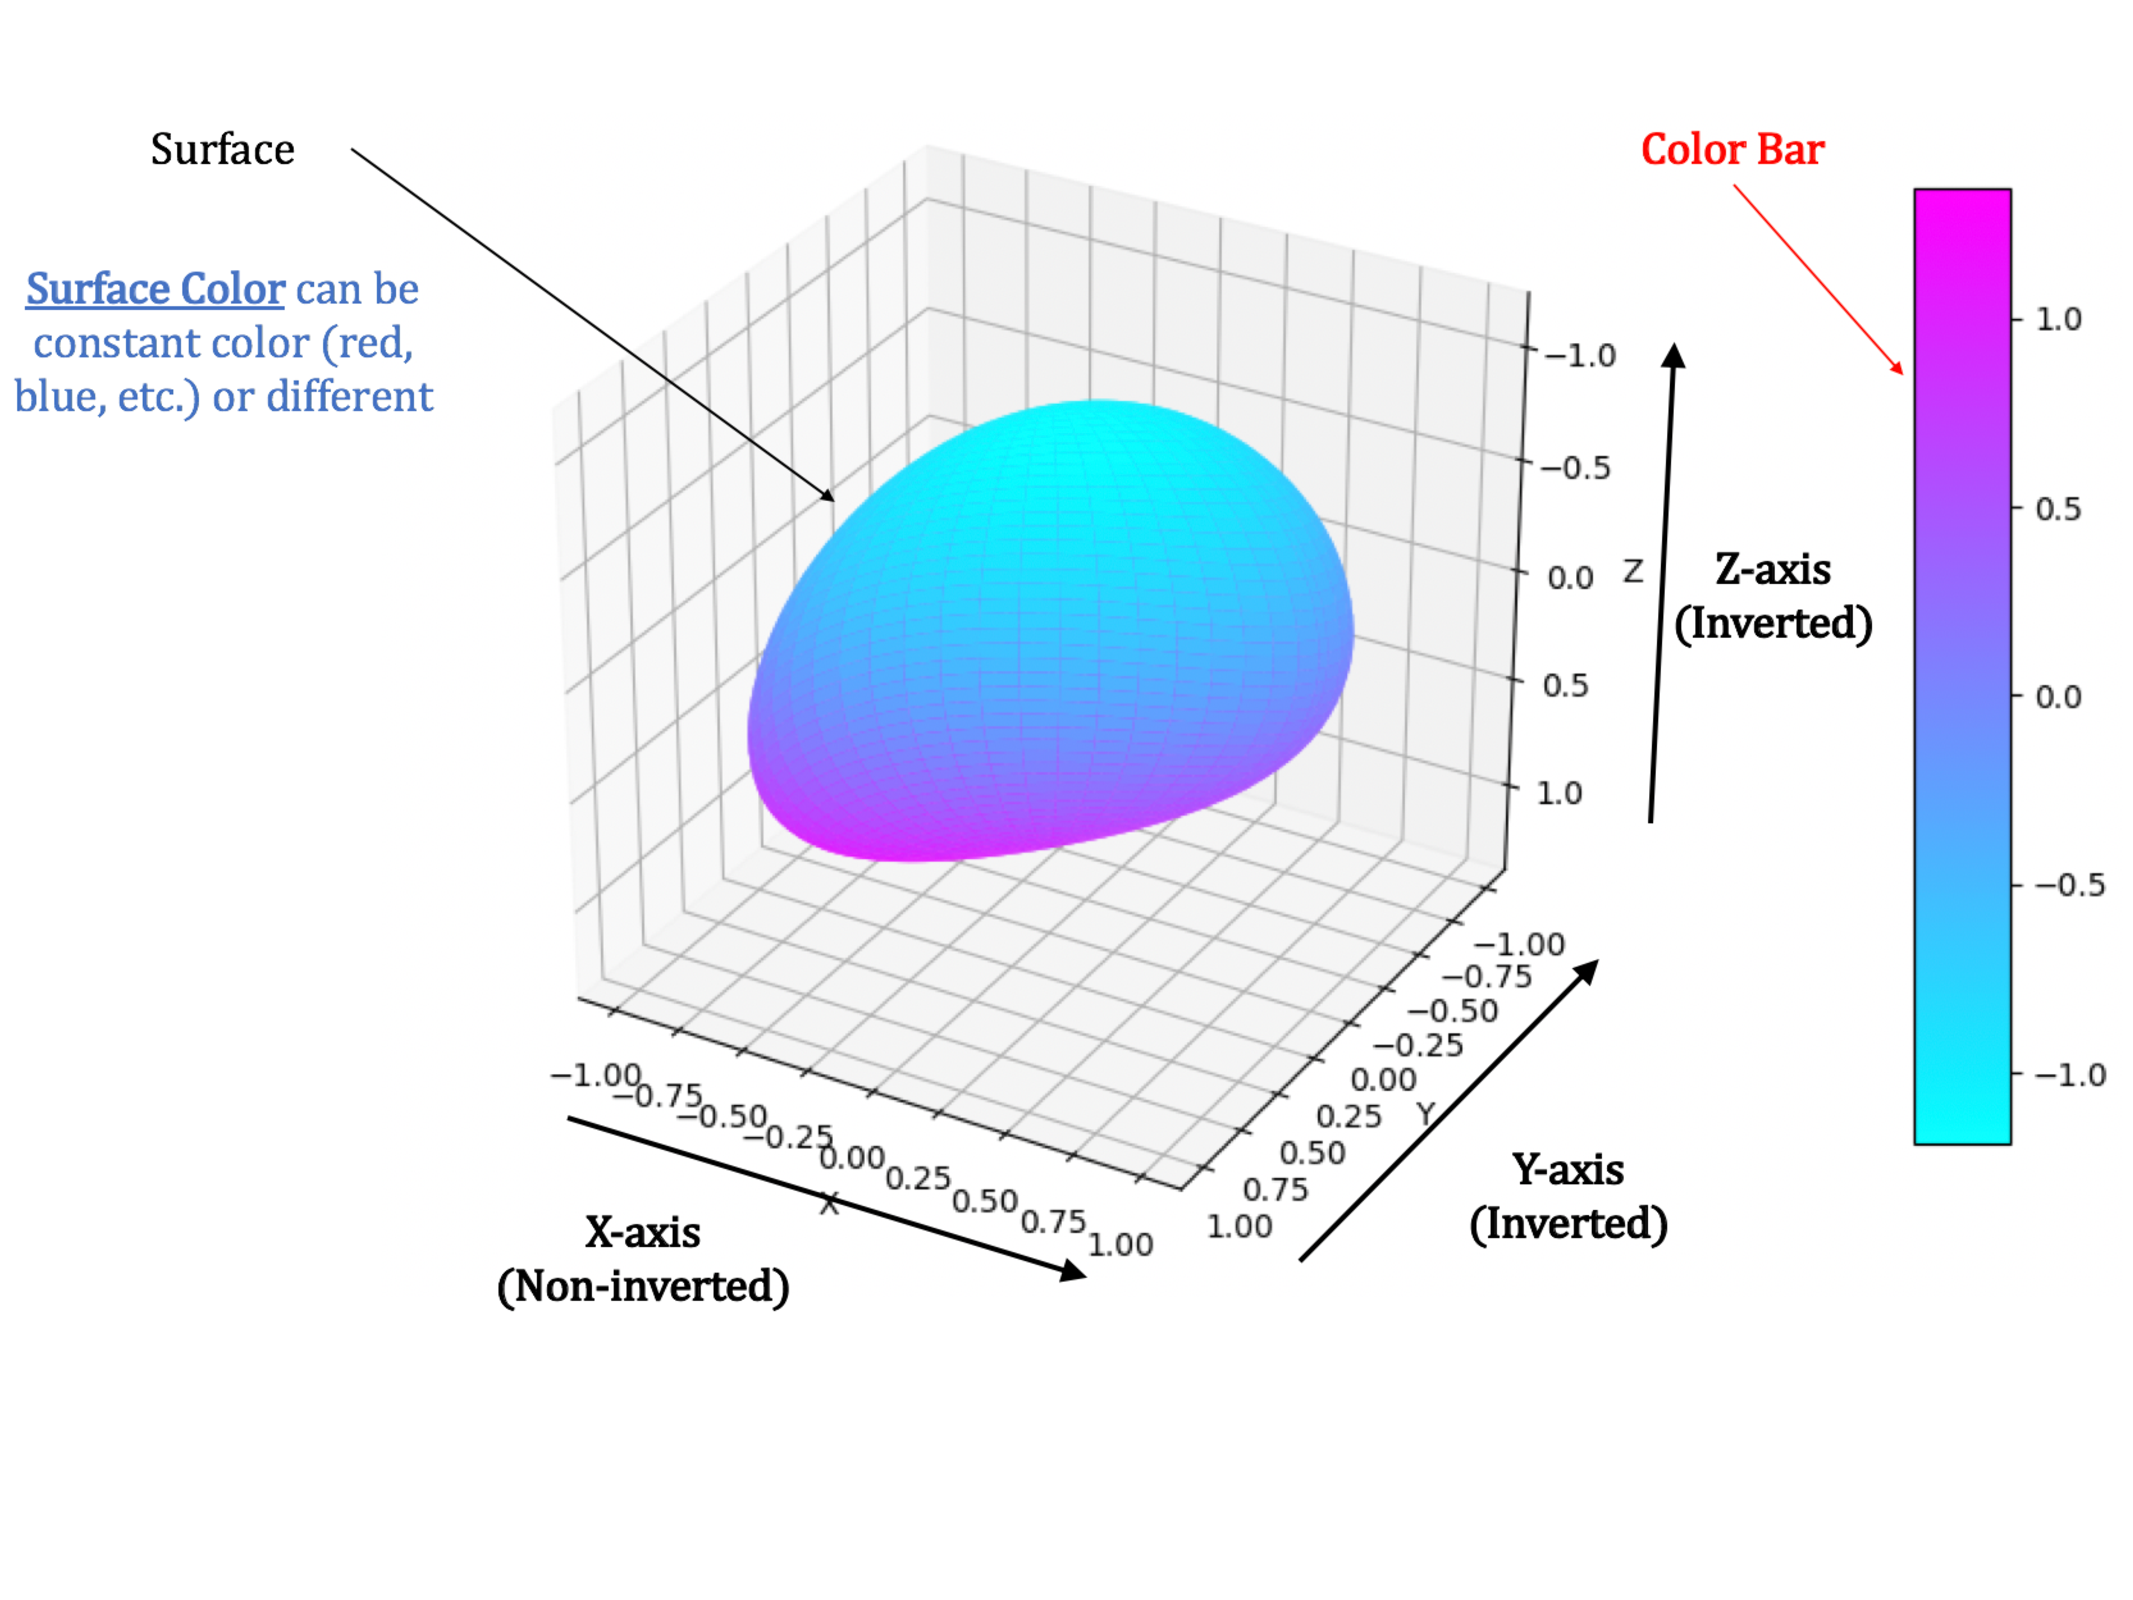
\includegraphics[width=0.52\linewidth]{figs/il-full-3d.pdf}
    % \vspace{-1.6cm}
    \label{fig:3d}}

\caption{Illustration of two of ChartDialog plot types. \textbf{(a)} \textbf{Line Chart} has slots such as \textit{Line Style, Marker Interval}.
\textbf{ (b)} A \textbf{3D Surface}  has slots such as \textit{Surface Color}.
}
\label{fig:slotsfortwo}
\end{figure}


\begin{table}[h]
\centering
\resizebox{\linewidth}{!}{%
\begin{tabular}{|l|l|l|}
\hline
& Plot Types & Slots \\
\hline
1. & Axes & Polarize, X-axis Scale, Y-axis Scale, X-axis Position, Y-axis Position, Invert X-axis, Invert Y-axis,\\
& & Grid Line Type, Grid Line Style,Grid Line Width, Grid Line Color, Font Size \\
\hline
2. & 3D Surface & Color map, Invert X-axis, Invert Y-Axis, Invert Z-Axis   \\
\hline
3. & Bar Chart & Bar Orientation, Bar Height, Bar Face Color, Bar Edge Width, Bar Edge Color,  Show Error Bar,  \\
& & Error Bar Color, Error Bar Cap Size, Error Bar, Cap Thickness, Data Series Name \\
\hline
4. & Contour/Filled & Contour Plot Type, Number of levels, Color Map, Color Bar Orientation, Color Bar \\
& &  Length, Color Bar Thickness  \\
\hline
5. & Contour/Lined & Contour Plot Type, Lined Style, Line Width\\ 
\hline
6. & Histogram &  Number of Bins, Bar Relative Width, Bar Face Color, Bar Edge Width, Bar Edge \\
& & Color, Data Series Name \\
\hline
7. & Matrix &  Color Map, Invert X-axis, Invert Y-axis \\
\hline
8. & Line Chart &  Line Style, Line Width, Line Color, Marker Type, Marker Size, Marker Face Color,  \\
& & Marker Edge Color, Marker Interval, Data Series Name, Show Error Bar, Error Bar Color,\\
& & Error Bar Cap Size, Error Bar Cap Thickness \\
\hline
9. & Pie Chart &  Exploding Effect, Precision Digits, Percentage tags’ distance from center, \\ 
& & Label tag’s distance from center, Radius, Section Edge Width, Section Edge Color
 \\
\hline
10. & Polar & Polarize, Grid Line Type, Grid Line Style, Grid Line Width, Grid Line Color, Font Size \\
\hline
11. & Scatter &  Polarize, Marker Type, Marker Size, Marker Face Color, Marker Edge Width, Marker Edge Color,  \\
& &   Color  Map, Color Bar Orientation, Color Bar Length Color Bar Thickness
 \\
\hline
12. &Streamline & Density, Line Width, Line Color, Color Map, Arrow Size, Arrow Style  \\
\hline
\end{tabular}
}
\caption{Plot types and slots in our dataset}
\label{tbl:chartdialogs-onto}
\end{table}


\subsubsection{Dataset Overview}
To enable training neural models for the new task, we collected a dataset, \textit{ChartDialogs}, which consists of actual human dialogs on completing plotting tasks. 
We used Amazon Mechanical Turk for dataset collection. For each dialog, we engage two workers simultaneously to play the \textit{user} and \textit{system} respectively, and randomly generate a \textit{target plot}. The target plot is only visible to the user worker. It stands for the plot that an actual user wants in real world scenarios. During the dialog, the user worker has to describe the plot to the system worker to accurately reproduce the exact plot to complete the task.
% \yutong{include the task screenshot and dataset statistics?}

\subsubsection{Methods}
We assessed the performance of various methods for training TOD system on our ChartDialogs dataset.
We experimented with two categories of methods: S2S-based and classification-based.
For S2S-based methods, we linearize the dialog state in similar manner with previous work~\cite{sequicity}. The model takes as input the user utterance and linearized dialog state, and predicts a linearized \textit{dialog state update}, which includes the slot values that should be updated. We use LSTM as both encoder and decoder architecture for the S2S model.
For classification-based methods, we exploit the specific design of our domain ontology that the possible values of each slot come from a finite value pool. Thus, we can treat dialog state tracking as a classification problem for each slot separately. The input format is the same as above, i.e. the concatenation of user utterance and linearized dialog state. We experimented using bag-of-word, LSTM and BERT~\cite{bert} as input encoding methods, and train a logistic-regression or multi-layer perceptron (MLP) classifier heads\footnote{An MLP consists of several fully-connected layers with non-linear activation functions, finally applying a softmax layer to predict the probabilities of each class.} for each slot on top of the encoded input representation.
In detail, we try three different classification methods: (i) \textbf{MaxEnt}, using bag-of-word embedding and logistic regression classifier; (ii) \textbf{LSTM+MLP}, using LSTM as input encoder and MLP classifier heads; and (iii) \textbf{BERT+MLP}, using BERT (parameters frozen) as input encoder and MLP classifier heads.
% An illustration of the input-output formulation is provided in Figure~\ref{chartdialog-IO}.

As a relevant detail, we experimented using different \textit{granularity} for dialog state linearization, SPLIT, SINGLE and PAIR, detailed in Table~\ref{tbl:chartdialogs-granu}. Conceptually, SPLIT best leverages the semantic overlap between different slots and values, while PAIR is the most succinct with regard to sequence length. In the result section, we shed light on how this design choice influences the model performances.


\begin{table}[h]
\centering
\resizebox{\linewidth}{!}{%
\begin{tabular}{|l|l|l|}
\hline
Granularity		& Description	& Example \\\hline
(Dialog state)	& The dialog state to linearize	& \texttt{(plot\_type = line chart, line\_color = blue, marker\_type = circle)}	\\
\hline\hline
PAIR 		& Combined slot-value pair as a token 	& ``plot\_type:line\_chart~~line\_color:blue~~marker\_type:circle'' \\\hline
SINGLE 		& Each slot or value as a single token 	& ``plot\_type~~line\_chart~~line\_color~~blue~~marker\_type~~circle'' \\\hline
SPLIT 		& Split slot or values into natural language tokens 	& ``plot type : line chart | line color : blue | marker type : circle'' \\\hline
\end{tabular}
}
\caption{Explanation of dialog state linearization granularity.}
\label{tbl:chartdialogs-granu}
\end{table}


\subsubsection{Experiments}
\paragraph{Evaluation Metrics} We evaluate the model performance on a turn-based manner, i.e. use each dialog turn as a data point and compare the model prediction with ground truth (human worker choices). For evaluation metrics, we use \textit{exact match rate} which is the proportion of dialog state predictions fully matching the ground truth; and \textit{Slot-F1} which measures the performance on slot-level.\footnote{We use F1-score instead of accuracy because in most cases, most slots are inactive and have the \textit{[None]} value. That causes uneven distributions among slot values, thus we use F1-score.}

\paragraph{Results} The main results are shown in Table~\ref{tbl:chartdialogs-res}. The S2S method largely outperforms classification-based methods, despite the fact that classification-based methods exploit the domain-specific design. Our hypothesis is that, the sequence predictor (decoder) in S2S model learns implicit inter-dependencies between slots (e.g. certain slots are only active for certain plot types), while the separated classifiers do not.
Comparing classification methods, the simplest method, MaxEnt (with PAIR granularity) is competitive and outperforms baseline neural models. The unsatisfactory performance is possibly because their non-robustness or overfitting to noises in the dataset.

Based on the best-performing S2S method, we also conducted ablation study to verify the usefulness of user utterance and dialog state in the input. User utterances are useful as expected, as without user utterances the prediction would be an educated guess. The dialog states are also useful, which is a positive sign for the importance of (internal) structured data in TOD. Intuitively, the benefits of dialog state could be to provide a better semantic context, i.e. more relevant information, for the model.
Comparing the linearization granularity for the S2S model, the SINGLE setting performs the best. It possibly implies that, among the three granularity settings, SINGLE achieves a proper trade-off between capturing slot / value semantics and controlling the sentence length.

\begin{table}[t]
\centering
% yutong: \resizebox is not working properly with pdfLatex, unsure why 
\resizebox{0.7\linewidth}{!}{%
\begin{tabular}{|l|c|c|c|c|c|c|}
\hline
\multirow{2}{*}{Methods} & \multicolumn{3}{c|}{Exact Match} & \multicolumn{3}{c|}{Slot F1} \\
\cline{2-7}
& SPLIT & SINGLE & PAIR & SPLIT & SINGLE & PAIR \\
\hline
% S2S-PLOT+TXT & 0.585 & \textbf{0.613} & 0.594 & 0.871 & \textbf{0.890} & 0.888 \\
% \hline
S2S     & 0.601 & \textbf{0.613} & 0.591 & 0.874 & \textbf{0.893} & 0.885 \\
\hline
S2S-NoState & 0.525 & 0.549 & 0.535 & 0.847 & 0.866 & 0.863 \\
\hline
S2S-NoUtterance & 0.060 & 0.047 & 0.046 & 0.316 & 0.306 & 0.155 \\
\hline
MaxEnt  & 0.196 & 0.265 & \textbf{\textit{0.422}} & 0.677 & 0.734 & \textbf{\textit{0.806}} \\
\hline
LSTM+MLP & 0.328 & 0.324 & 0.325 & 0.714 & 0.712 & 0.724 \\
\hline
BERT+MLP & 0.311 & n/a\tablefootnote{Due to the word-piece tokenization used in BERT, the SINGLE and PAIR linearizations are also tokenized to granularity level of SPLIT, therefore we do not report their performance.\label{footnote-BERT}} & n/a\textsuperscript{\ref{footnote-BERT}} & 0.723 & n/a\textsuperscript{\ref{footnote-BERT}} & n/a\textsuperscript{\ref{footnote-BERT}} \\
\hline
\end{tabular}
}
% \vspace{-0.7cm}
\caption{Exact match plotting performance.}
\label{tbl:chartdialogs-res}
\end{table}


\section{Conclusion}
In this paper, we reviewed relevant tasks of natural language interfaces, semantic parsing (focusing on text-to-SQL) and task-oriented dialog (TOD) systems. We survey representative methods on these tasks, especially focusing on the perspective of representing and incorporating structured data, both external and internal. In general, linearization methods are widely adopted. They are applicable for almost all types of structured data while exhibiting competitive performances. Nonetheless, for  different types of structured data, there are still opportunities for further performance gains by designing methods that capitalize on their distinct properties.
We also present our original studies on the relevant tasks, and discuss our findings regarding the topic of structured data representation.

For future work on NLIs and structured data representation, many opportunities and challenges are still  ripe for exploration. Despite the increasing performance on benchmarks, neural-based NLIs are still not widely deployed in the real world. Identifying and analyzing the challenges that remain when porting to  new domains, tasks, datasets or real-world scenarios is one line of future work.  Another future direction is a systematic study to find similarities among a subset of different tasks, or even all NLI-related tasks, to develop methods that are generalizable to new tasks with similar properties. Furthermore,  obtaining data for NLIs in new domains, even a small amount of data for few-shot or fine-tuning remains a time-consuming  endeavor that requires complex crowd-sourcing pipelines, and can be expensive.   Coming up with ways to quickly obtain new data for training NLIs in new domains, and tasks  is another direction for future work. 

% Figure
% \begin{figure}
% 
\includegraphics{figs/myfigure.png}
% \caption{A simple figure.}
% \end{figure}

% Bib
\begin{thebibliography}{10}
\itemsep=1pt
\begin{small}

\bibitem{winograd1971procedures} Winograd, Terry. “Procedures As A Representation For Data In A Computer Program For Understanding Natural Language.” (1971).

\bibitem{karamcheti-etal-2020-learning} Karamcheti, Siddharth, Dorsa Sadigh and Percy Liang. “Learning Adaptive Language Interfaces through Decomposition.” ArXiv abs/2010.05190 (2020): n. pag.

\bibitem{GeoQuery:Zelle1996LearningTP} Zelle, John M. and Raymond J. Mooney. “Learning to Parse Database Queries Using Inductive Logic Programming.” AAAI/IAAI, Vol. 2 (1996).

\bibitem{WTQ} Pasupat, Panupong and Percy Liang. “Compositional Semantic Parsing on Semi-Structured Tables.” ArXiv abs/1508.00305 (2015): n. pag.

\bibitem{Artzi2013UWSPF} Artzi, Yoav and Luke Zettlemoyer. “UW SPF: The University of Washington Semantic Parsing Framework.” ArXiv abs/1311.3011 (2013): n. pag.

\bibitem{Dong2016LanguageTL} Dong, Li and Mirella Lapata. “Language to Logical Form with Neural Attention.” ArXiv abs/1601.01280 (2016): n. pag.

\bibitem{Dong2018CoarsetoFineDF} Dong, Li and Mirella Lapata. “Coarse-to-Fine Decoding for Neural Semantic Parsing.” ACL (2018).

\bibitem{Cheng2019LearningAE} Cheng, Jianpeng, Siva Reddy, Vijay A. Saraswat and Mirella Lapata. “Learning an Executable Neural Semantic Parser.” Computational Linguistics 45 (2019): 59-94.

\bibitem{yu2018spider} Yu, Tao, Rui Zhang, Kai-Chou Yang, Michihiro Yasunaga, Dongxu Wang, Zifan Li, James Ma, Irene Z Li, Qingning Yao, Shanelle Roman, Zilin Zhang and Dragomir R. Radev. “Spider: A Large-Scale Human-Labeled Dataset for Complex and Cross-Domain Semantic Parsing and Text-to-SQL Task.” EMNLP (2018).

\bibitem{tapas} Herzig, Jonathan, Pawel Krzysztof Nowak, Thomas Müller, Francesco Piccinno and Julian Martin Eisenschlos. “TaPas: Weakly Supervised Table Parsing via Pre-training.” ArXiv abs/2004.02349 (2020): n. pag.

\bibitem{tableformer} Yang, Jingfeng, Aditya Gupta, Shyam Upadhyay, Luheng He, Rahul Goel and Shachi Paul. “TableFormer: Robust Transformer Modeling for Table-Text Encoding.” ArXiv abs/2203.00274 (2022): n. pag.

\bibitem{picard} Scholak, Torsten, Nathan Schucher and Dzmitry Bahdanau. “PICARD: Parsing Incrementally for Constrained Auto-Regressive Decoding from Language Models.” ArXiv abs/2109.05093 (2021): n. pag.

\bibitem{uskg} Xie, Tianbao, Chen Henry Wu, Peng Shi, Ruiqi Zhong, Torsten Scholak, Michihiro Yasunaga, Chien-Sheng Wu, Ming Zhong, Pengcheng Yin, Sida I. Wang, Victor Zhong, Bailin Wang, Chengzu Li, Connor Boyle, Ansong Ni, Ziyu Yao, Dragomir Radev, Caiming Xiong, Lingpeng Kong, Rui Zhang, Noah A. Smith, Luke Zettlemoyer and Tao Yu. “UnifiedSKG: Unifying and Multi-Tasking Structured Knowledge Grounding with Text-to-Text Language Models.” ArXiv abs/2201.05966 (2022): n. pag.

\bibitem{bridge} Lin, Xi Victoria, Richard Socher and Caiming Xiong. “Bridging Textual and Tabular Data for Cross-Domain Text-to-SQL Semantic Parsing.” EMNLP Findings (2020).

\bibitem{grappa} Yu, Tao, Chien-Sheng Wu, Xi Victoria Lin, Bailin Wang, Yi Chern Tan, Xinyi Yang, Dragomir Radev, Richard Socher and Caiming Xiong. “GraPPa: Grammar-Augmented Pre-Training for Table Semantic Parsing.” ArXiv abs/2009.13845 (2021): n. pag.

\bibitem{tabert} Yin, Pengcheng, Graham Neubig, Wen-tau Yih and Sebastian Riedel. “TaBERT: Pretraining for Joint Understanding of Textual and Tabular Data.” ArXiv abs/2005.08314 (2020): n. pag.

\bibitem{schema-gnn} Bogin, Ben, Matt Gardner and Jonathan Berant. “Representing Schema Structure with Graph Neural Networks for Text-to-SQL Parsing.” ArXiv abs/1905.06241 (2019): n. pag.

\bibitem{lgesql} Cao, Ruisheng, Lu Chen, Zhi Chen, Yanbin Zhao, Su Zhu and Kai Yu. “LGESQL: Line Graph Enhanced Text-to-SQL Model with Mixed Local and Non-Local Relations.” ACL (2021).

\bibitem{ratsql} Wang, Bailin, Richard Shin, Xiaodong Liu, Oleksandr Polozov and Matthew Richardson. “RAT-SQL: Relation-Aware Schema Encoding and Linking for Text-to-SQL Parsers.” ACL (2020).

\bibitem{s2sql} Hui, Binyuan, Ruiying Geng, Lihan Wang, Bowen Qin, Bowen Li, Jian Sun and Yongbin Li. “S2SQL: Injecting Syntax to Question-Schema Interaction Graph Encoder for Text-to-SQL Parsers.” ArXiv abs/2203.06958 (2022): n. pag.

\bibitem{ASR-Reranker} Weng, Yue, Sai Sumanth Miryala, Chandra Khatri, Runze Wang, Huaixiu Zheng, Piero Molino, Mahdi Namazifar, Alexandros Papangelis, Hugh Williams, Franziska Bell and Gokhan Tur. “Joint Contextual Modeling for ASR Correction and Language Understanding.” ICASSP 2020 - 2020 IEEE International Conference on Acoustics, Speech and Signal Processing (ICASSP) (2020): 6349-6353.

\bibitem{ASR-S2S} Mani, Anirudh, Shruti Palaskar, Nimshi Venkat Meripo, Sandeep Konam and Florian Metze. “ASR Error Correction and Domain Adaptation Using Machine Translation.” ICASSP 2020 - 2020 IEEE International Conference on Acoustics, Speech and Signal Processing (ICASSP) (2020): 6344-6348.

\bibitem{bAbIDialog} Bordes, Antoine and Jason Weston. “Learning End-to-End Goal-Oriented Dialog.” ArXiv abs/1605.07683 (2017): n. pag.

\bibitem{airdialogue} Wei, Wei, Quoc V. Le, Andrew M. Dai and Jia Li. “AirDialogue: An Environment for Goal-Oriented Dialogue Research.” EMNLP (2018).

\bibitem{DSTC2} Henderson, Matthew, Blaise Thomson and J. Williams. “The Second Dialog State Tracking Challenge.” SIGDIAL Conference (2014).

\bibitem{multiwoz} Budzianowski, Paweł, Tsung-Hsien Wen, Bo-Hsiang Tseng, Iñigo Casanueva, Stefan Ultes, Osman Ramadan and Milica Gasic. “MultiWOZ - A Large-Scale Multi-Domain Wizard-of-Oz Dataset for Task-Oriented Dialogue Modelling.” EMNLP (2018).

\bibitem{Zhang2020RecentAA} Zhang, Zheng, Ryuichi Takanobu, Minlie Huang and Xiaoyan Zhu. “Recent Advances and Challenges in Task-oriented Dialog System.” ArXiv abs/2003.07490 (2020): n. pag.


% \bibitem{wen2017EndtoEnd} Tsung-Hsien Wen, David Vandyke, Nikola Mrkšić, Milica Gašić, Lina M. Rojas-Barahona, Pei-Hao Su, Stefan Ultes, and Steve Young. 2017. A Network-based End-to-End Trainable Task-oriented Dialogue System. In Proceedings of the 15th Conference of the European Chapter of the Association for Computational Linguistics: Volume 1, Long Papers, pages 438–449, Valencia, Spain. Association for Computational Linguistics.

\bibitem{wen2017EndtoEnd} Rojas-Barahona, Lina Maria, Milica Gašić, Nikola Mrksic, Pei-hao Su, Stefan Ultes, Tsung-Hsien Wen, Steve J. Young and David Vandyke. “A Network-based End-to-End Trainable Task-oriented Dialogue System.” EACL (2017).

\bibitem{liu2018DialogueHumanTeaching} Liu, Bing, Gökhan Tür, Dilek Z. Hakkani-Tür, Pararth Shah and Larry Heck. “Dialogue Learning with Human Teaching and Feedback in End-to-End Trainable Task-Oriented Dialogue Systems.” NAACL (2018).

\bibitem{zhang2020LatentBeliefState} Zhang, Yichi, Zhijian Ou, Huixin Wang and Junlan Feng. “A Probabilistic End-To-End Task-Oriented Dialog Model with Latent Belief States towards Semi-Supervised Learning.” ArXiv abs/2009.08115 (2020): n. pag.

\bibitem{mem2seq} Madotto, Andrea, Chien-Sheng Wu and Pascale Fung. “Mem2Seq: Effectively Incorporating Knowledge Bases into End-to-End Task-Oriented Dialog Systems.” ACL (2018).

\bibitem{wmm2seq} Chen, Xiuyi, Jiaming Xu and Bo Xu. “A Working Memory Model for Task-oriented Dialog Response Generation.” ACL (2019).

\bibitem{sequicity} Lei, Wenqiang, Xisen Jin, Min-Yen Kan, Zhaochun Ren, Xiangnan He and Dawei Yin. “Sequicity: Simplifying Task-oriented Dialogue Systems with Single Sequence-to-Sequence Architectures.” ACL (2018).

\bibitem{ham2020-gpt2-tod} Ham, Dong-hyun, Jeong-Gwan Lee, Youngsoo Jang and Kyungmin Kim. “End-to-End Neural Pipeline for Goal-Oriented Dialogue Systems using GPT-2.” ACL (2020).

\bibitem{chen2019SemanticallyConditioned} Chen, Wenhu, Jianshu Chen, Pengda Qin, Xifeng Yan and William Yang Wang. “Semantically Conditioned Dialog Response Generation via Hierarchical Disentangled Self-Attention.” ACL (2019).

\bibitem{moon2019OpenDialKG} Moon, Seungwhan, Pararth Shah, Anuj Kumar and Rajen Subba. “OpenDialKG: Explainable Conversational Reasoning with Attention-based Walks over Knowledge Graphs.” ACL (2019).

\bibitem{cohen2020ScalableNeural} Cohen, William W., Haitian Sun, R. Alex Hofer and Matthew A. Siegler. “Scalable Neural Methods for Reasoning With a Symbolic Knowledge Base.” ArXiv abs/2002.06115 (2020): n. pag.

\bibitem{tuan2022TowardsLI} Tuan, Yi-Lin, Sajjad Beygi, Maryam Fazel-Zarandi, Qiaozi Gao, Alessandra Cervone and William Yang Wang. “Towards Large-Scale Interpretable Knowledge Graph Reasoning for Dialogue Systems.” ArXiv abs/2203.10610 (2022): n. pag.

\bibitem{chartdialogs} Shao, Yutong and Ndapa Nakashole. “ChartDialogs: Plotting from Natural Language Instructions.” ACL (2020).

\bibitem{tensorflowNMT} M. Luong, E. Brevdo, and R. Zhao. Neural machine translation (seq2seq) tutorial. https://github.com/tensorflow/nmt, 2017.

\bibitem{seq2seq} Sutskever, Ilya, Oriol Vinyals and Quoc V. Le. “Sequence to Sequence Learning with Neural Networks.” NIPS (2014).

\bibitem{lstm} Hochreiter, Sepp and Jürgen Schmidhuber. “Long Short-Term Memory.” Neural Computation 9 (1997): 1735-1780.

\bibitem{gru} Cho, Kyunghyun, Bart van Merrienboer, Çaglar Gülçehre, Dzmitry Bahdanau, Fethi Bougares, Holger Schwenk and Yoshua Bengio. “Learning Phrase Representations using RNN Encoder–Decoder for Statistical Machine Translation.” EMNLP (2014).

\bibitem{bahdanauAttention} Bahdanau, Dzmitry, Kyunghyun Cho and Yoshua Bengio. “Neural Machine Translation by Jointly Learning to Align and Translate.” CoRR abs/1409.0473 (2015): n. pag.

\bibitem{luongAttention} Luong, Thang, Hieu Pham and Christopher D. Manning. “Effective Approaches to Attention-based Neural Machine Translation.” EMNLP (2015).

\bibitem{vaswaniTransformer} Vaswani, Ashish, Noam M. Shazeer, Niki Parmar, Jakob Uszkoreit, Llion Jones, Aidan N. Gomez, Lukasz Kaiser and Illia Polosukhin. “Attention is All you Need.” ArXiv abs/1706.03762 (2017): n. pag.

\bibitem{bert} Devlin, Jacob, Ming-Wei Chang, Kenton Lee and Kristina Toutanova. “BERT: Pre-training of Deep Bidirectional Transformers for Language Understanding.” ArXiv abs/1810.04805 (2019): n. pag.

\bibitem{gpt2} Radford, Alec, Jeff Wu, Rewon Child, David Luan, Dario Amodei and Ilya Sutskever. “Language Models are Unsupervised Multitask Learners.” (2019).



\end{small}
\end{thebibliography}

\end{document}
